\documentclass{beamer}
\usepackage[english]{babel}
\usepackage{unicode-math}
\usepackage{xunicode}
\usepackage{url}
\usepackage{graphicx}
\usepackage[justification=centering, labelfont=bf]{caption}
\usepackage{float}
\usepackage{pgfgantt}
\usepackage{marvosym}
\usepackage{siunitx}
\usepackage{multirow}
\usepackage{svg}
\usepackage{float}
\usepackage{tabularx}
\usepackage{tikz}
\usepackage{minted}
\def\Checkmark{\tikz\fill[scale=0.4](0,.35) -- (.25,0) -- (1,.7) -- (.25,.15) -- cycle;}
\usetheme{Antibes}
\setbeamertemplate{navigation symbols}{}
\captionsetup[figure]{labelformat=empty}
\setcounter{tocdepth}{1}
\title{Platform for massive multiplayer programming games}
\institute{Facultat d'Informàtica de Barcelona}
\author{Héctor Ramón Jiménez}
\date{January 28, 2016}
\begin{document}
\frame{\titlepage}
\begin{frame}{Overview}
\tableofcontents
\end{frame}
\section{Introduction}
\subsection{Programming games}
\begin{frame}{What is a programming game?}
A computer game where the player does not directly interact with the game. Instead, the player writes a computer program
    (\texttt{AI}) that plays it.
\begin{figure}[H]
\begin{center}
\noindent\resizebox{!}{130pt}{
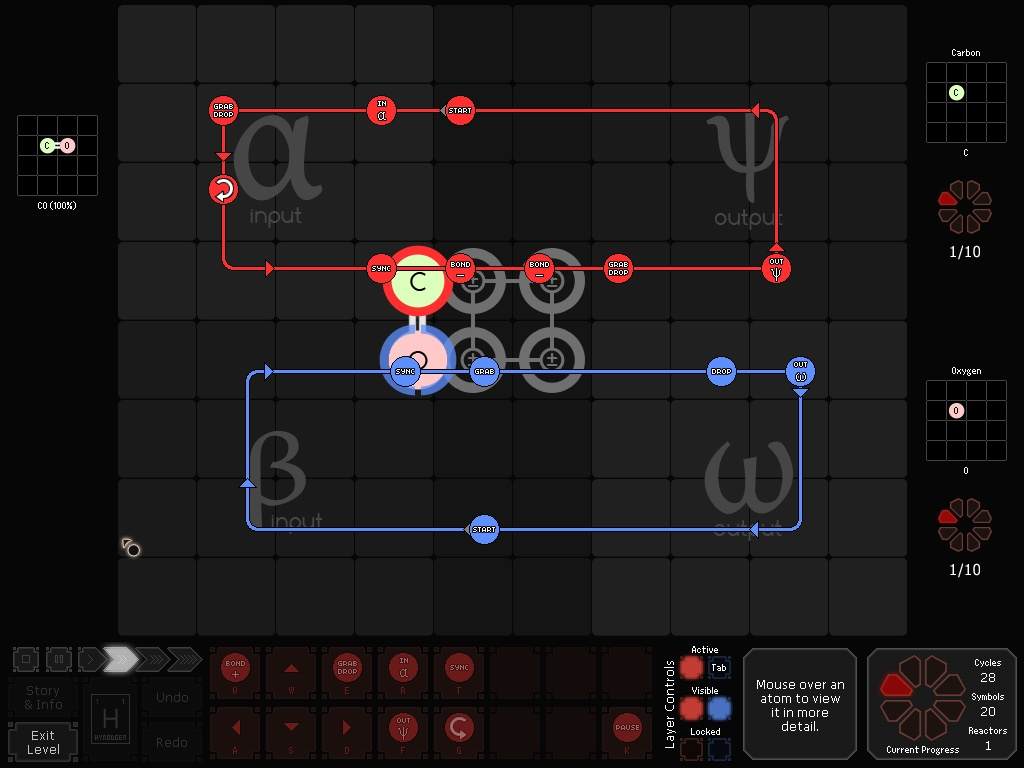
\includegraphics{images/spacechem.jpg}
}
\end{center}
\caption{SpaceChem}
\end{figure}
\end{frame}
\begin{frame}{Gamification}
Programming games can...
\begin{itemize}
\item
... show how algorithms work in a visual way.
\item
... motivate players to learn and improve.
\end{itemize}
For this reason, they are commonly used in education to teach students different programming techniques.
\end{frame}
\begin{frame}{The EDA competition}
An \texttt{AI} programming challenge held every semester at the FIB using \texttt{Jutge.org}
\begin{figure}[H]
\begin{center}
\noindent\resizebox{!}{60pt}{

\includegraphics{graphs/semafor.pdf}
}
\end{center}
\end{figure}
\end{frame}
\section{Formulation}
\subsection{Analysis}
\begin{frame}{The problem}
\begin{figure}[H]
\begin{center}
\noindent\resizebox{\textwidth}{!}{
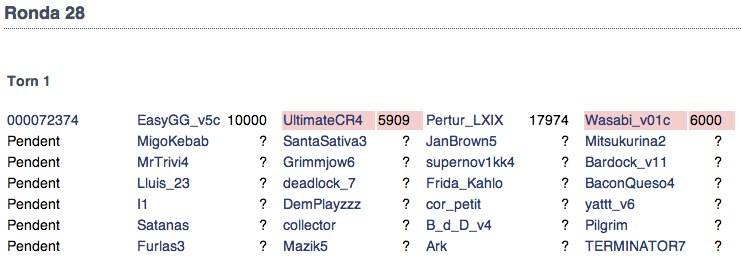
\includegraphics{images/jutge_rounds.png}
}
\end{center}
\caption{\texttt{Jutge.org} round system}
\end{figure}
\end{frame}
\begin{frame}{The problem}
\begin{figure}[H]
\begin{center}
\noindent\resizebox{!}{180pt}{
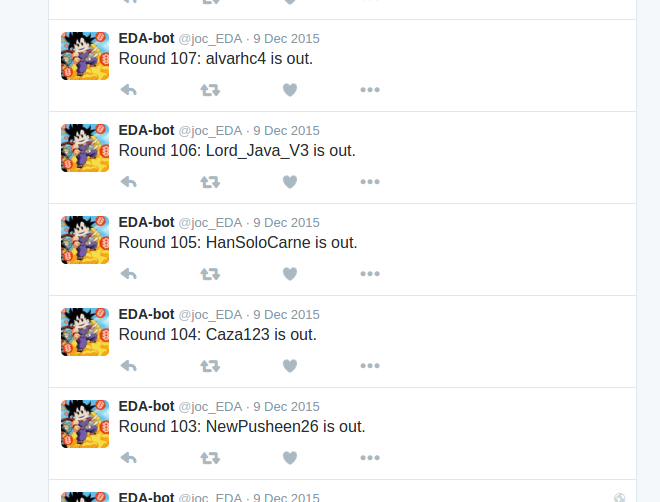
\includegraphics{images/eda_bot.png}
}
\end{center}
\caption{Twitter bot announcing eliminated players}
\end{figure}
\end{frame}
\begin{frame}{The state of the art}
\begin{itemize}
\item
Google's \texttt{AI} programming challenge
\item
Battlecode
\item
CodinGame
\item
\texttt{EDA} competition
\end{itemize}
All of them feature multiplayer programming games with a limited amount of players per match.
\end{frame}
\subsection{Objectives}
\begin{frame}{The main objective}
Develop a set of components that ease the creation and the usage of \emph{massive} multiplayer programming games (\texttt{MMPGs}).
\end{frame}
\begin{frame}{Secondary objectives}
\begin{enumerate}
\item
Develop an abstract game engine
\item
Allow hot-swapping of \texttt{AIs}
\item
Implement a real-time webviewer
\item
Make the infrastructure scalable and stable
\item
Create a game example
\end{enumerate}
\end{frame}
\begin{frame}{Main benefits}
\begin{itemize}
\item
For students:
\begin{itemize}
\item
Continuous learning process
\item
More attachment to the match
\item
More interesting games
\end{itemize}
\item
For professors:
\begin{itemize}
\item
Reduced amount of work
\item
No need to arrange multiple matches
\end{itemize}
\item
For game developers:
\begin{itemize}
\item
Easiness to build new \texttt{MMPGs}
\item
Freedom to create huge worlds
\end{itemize}
\end{itemize}
\end{frame}
\subsection{Design}
\begin{frame}{The solution}
\begin{center}
\noindent\resizebox{!}{180pt}{
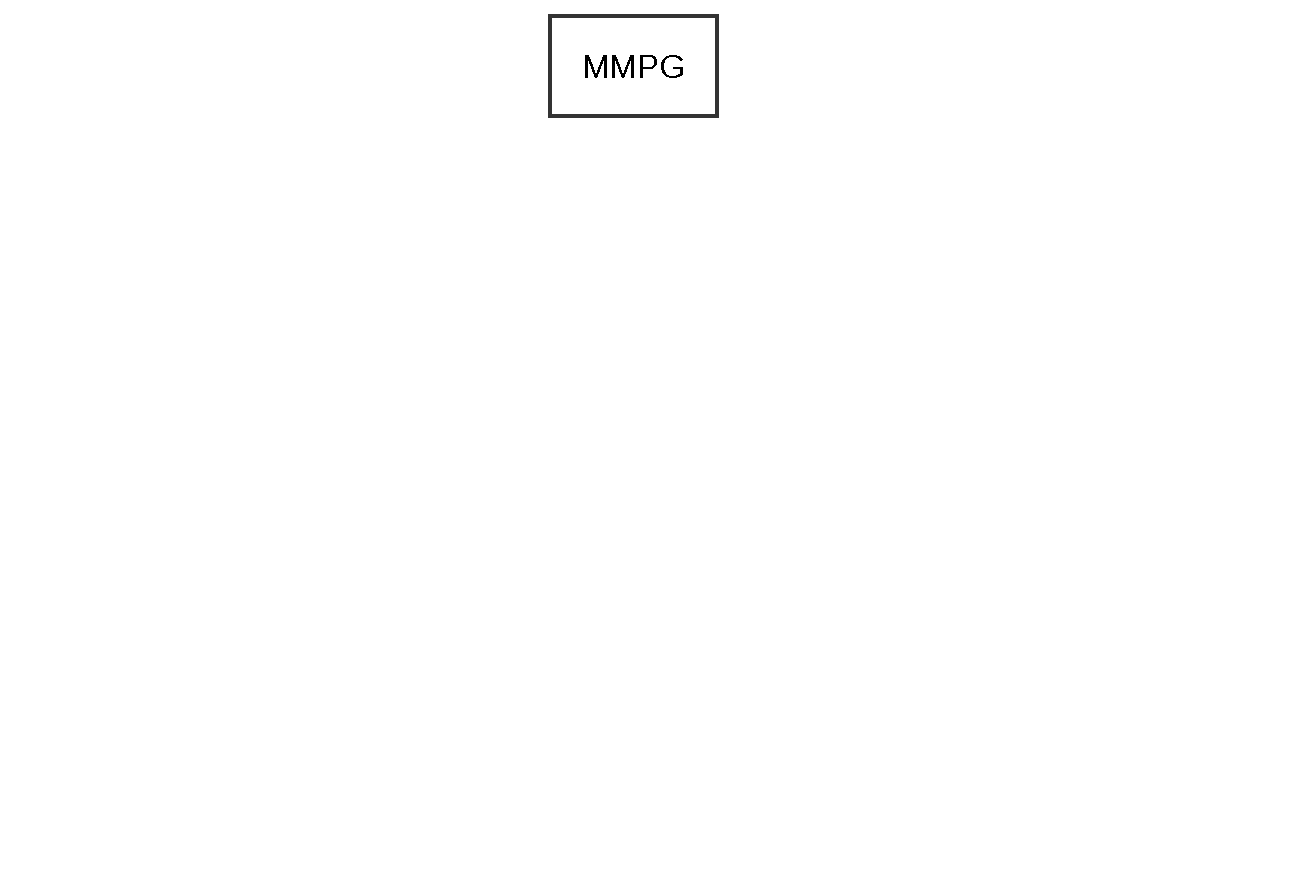
\includegraphics{graphs/mmpg_design_initial.pdf}
}
\end{center}
\end{frame}
\begin{frame}{The solution}
\begin{center}
\noindent\resizebox{!}{180pt}{
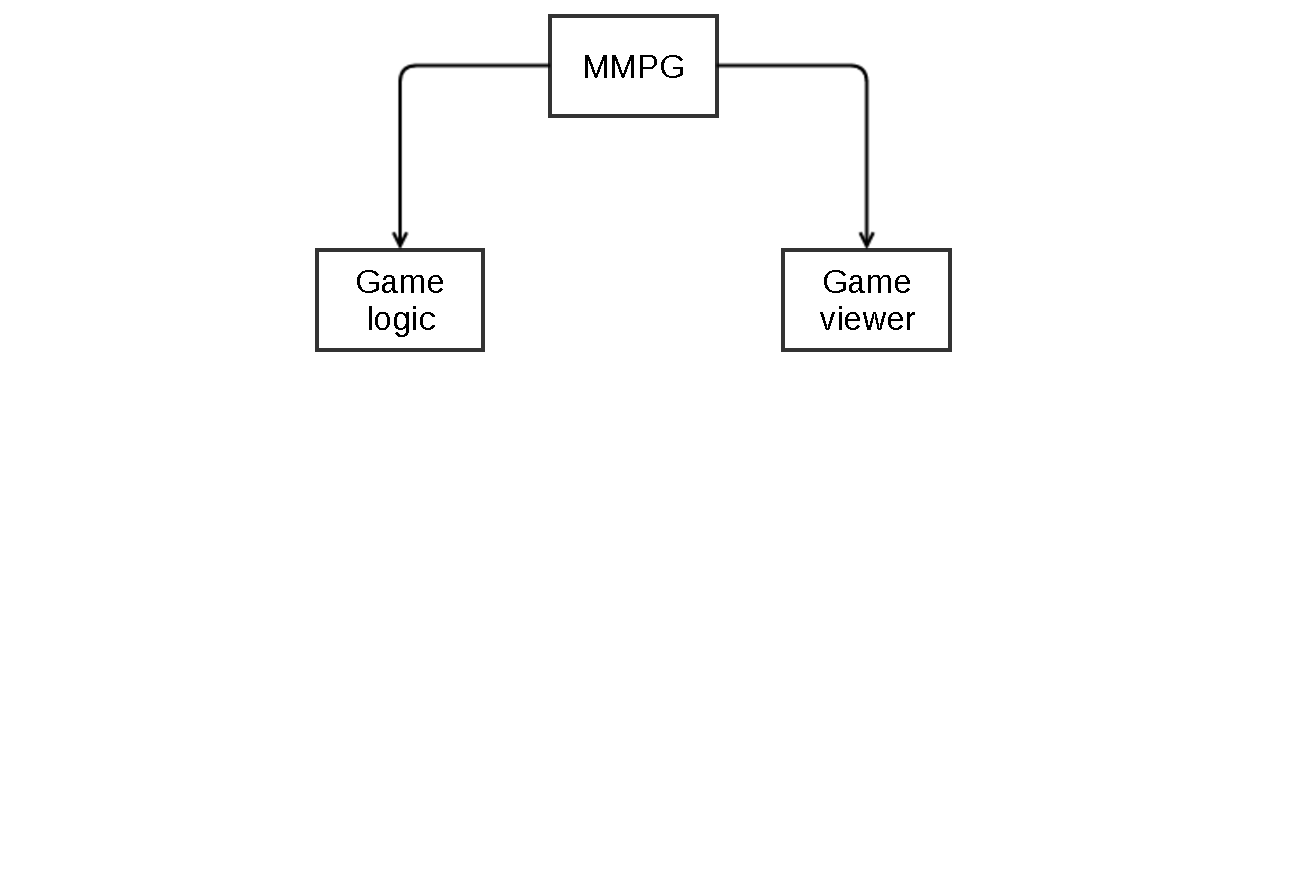
\includegraphics{graphs/mmpg_design_parts.pdf}
}
\end{center}
\end{frame}
\begin{frame}{The solution}
\begin{center}
\noindent\resizebox{!}{180pt}{
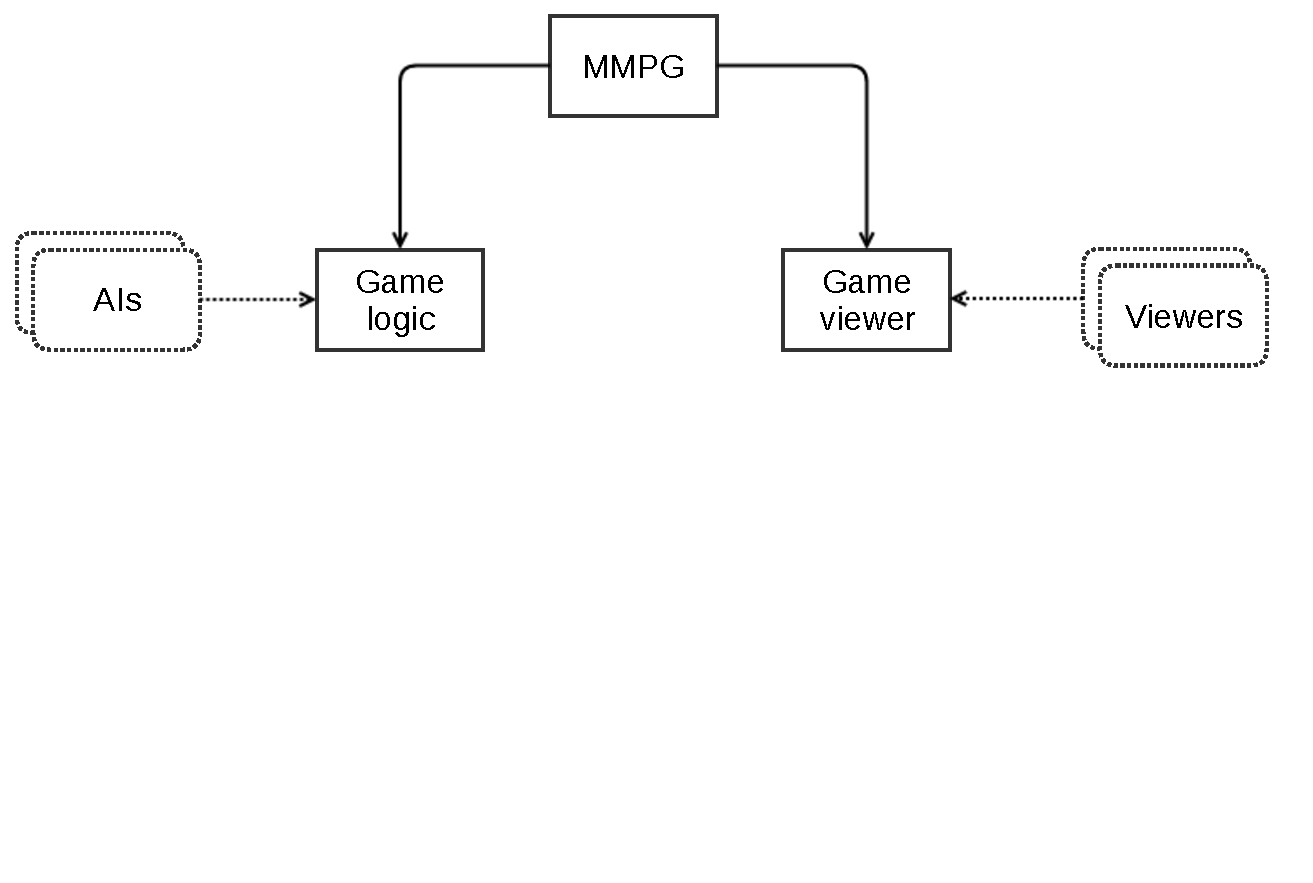
\includegraphics{graphs/mmpg_design_clients.pdf}
}
\end{center}
\end{frame}
\begin{frame}{The solution}
\begin{center}
\noindent\resizebox{!}{180pt}{
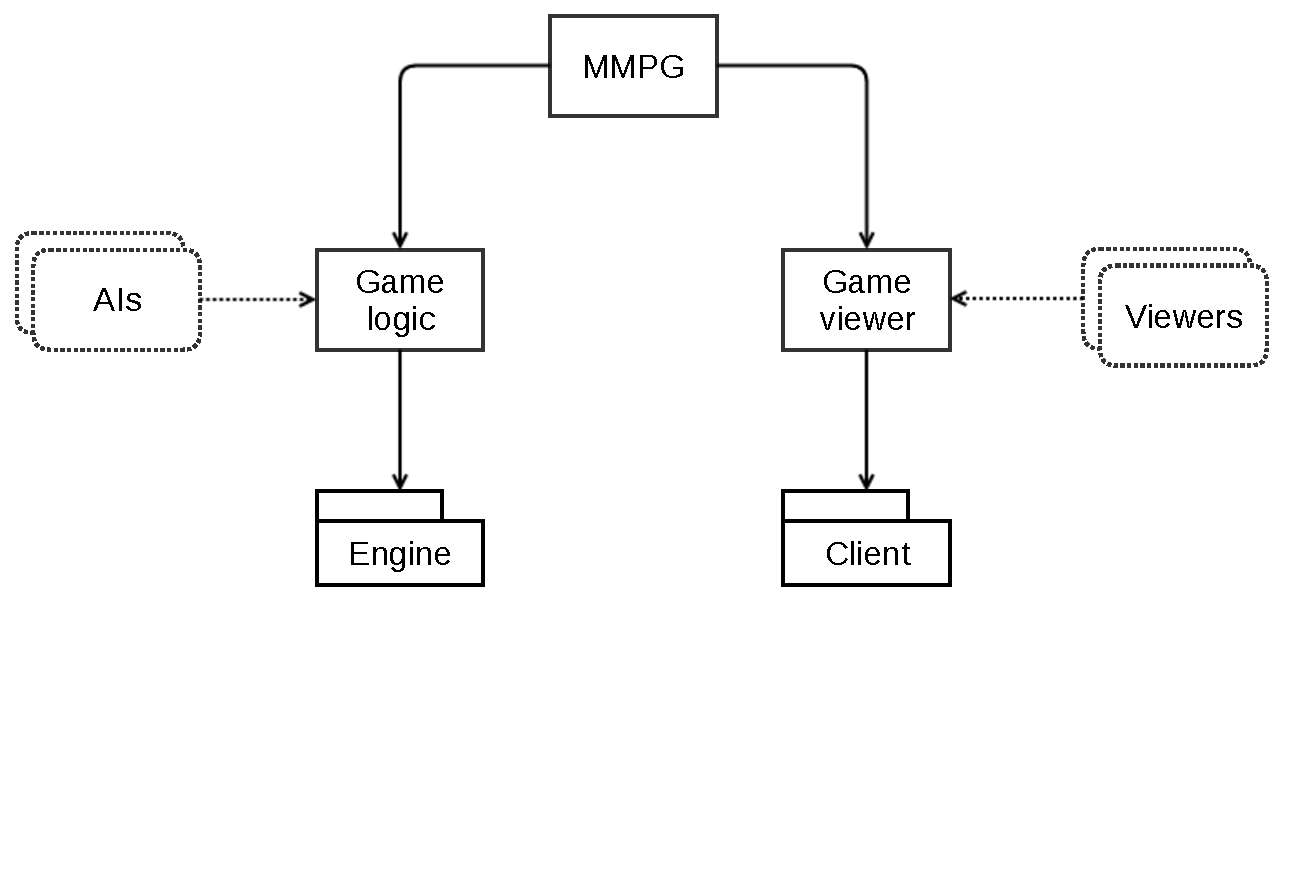
\includegraphics{graphs/mmpg_design_libs.pdf}
}
\end{center}
\end{frame}
\begin{frame}{The solution}
\begin{center}
\noindent\resizebox{!}{180pt}{
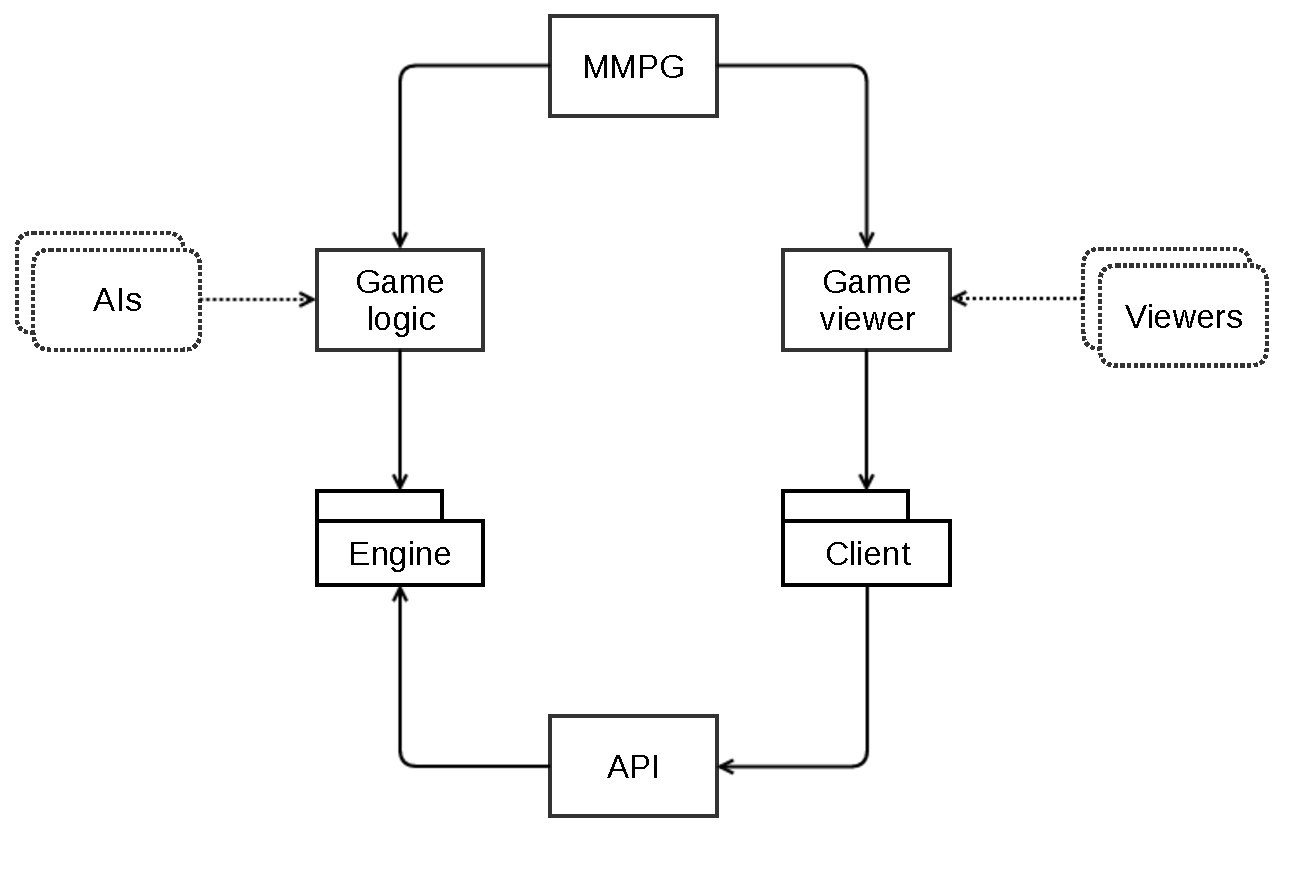
\includegraphics{graphs/mmpg_design.pdf}
}
\end{center}
\end{frame}
\section{Implementation}
\subsection{Methodology}
\begin{frame}{Continuous integration}
\begin{center}
\noindent\resizebox{!}{180pt}{
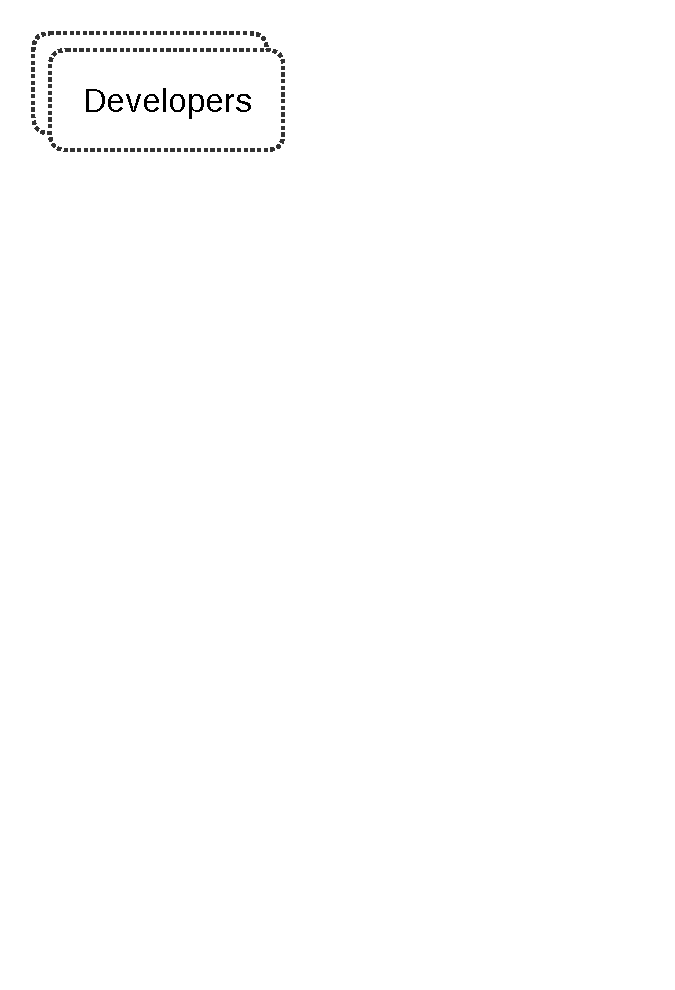
\includegraphics{graphs/ci_initial.pdf}
}
\end{center}
\end{frame}
\begin{frame}{Continuous integration}
\begin{center}
\noindent\resizebox{!}{180pt}{
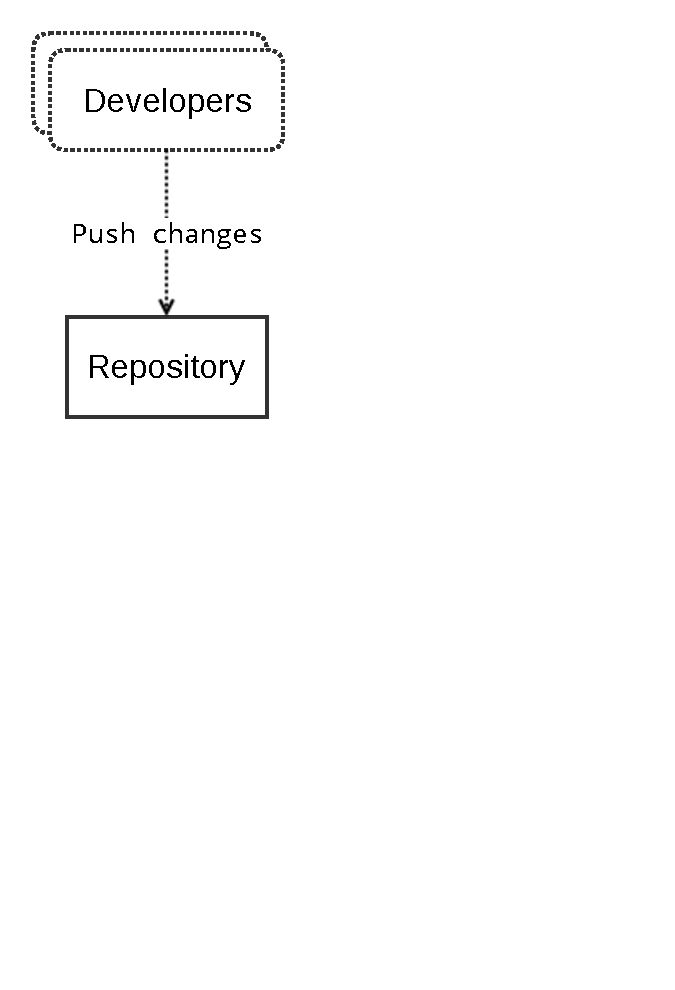
\includegraphics{graphs/ci_repo.pdf}
}
\end{center}
\end{frame}
\begin{frame}{Continuous integration}
\begin{center}
\noindent\resizebox{!}{180pt}{
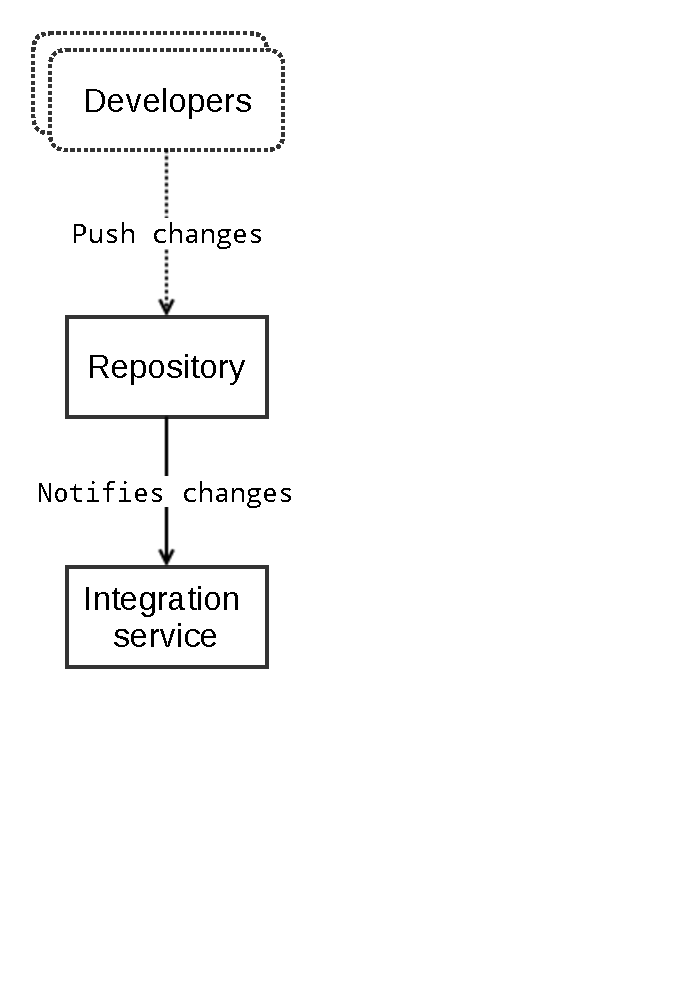
\includegraphics{graphs/ci_service.pdf}
}
\end{center}
\end{frame}
\begin{frame}{Continuous integration}
\begin{center}
\noindent\resizebox{!}{180pt}{
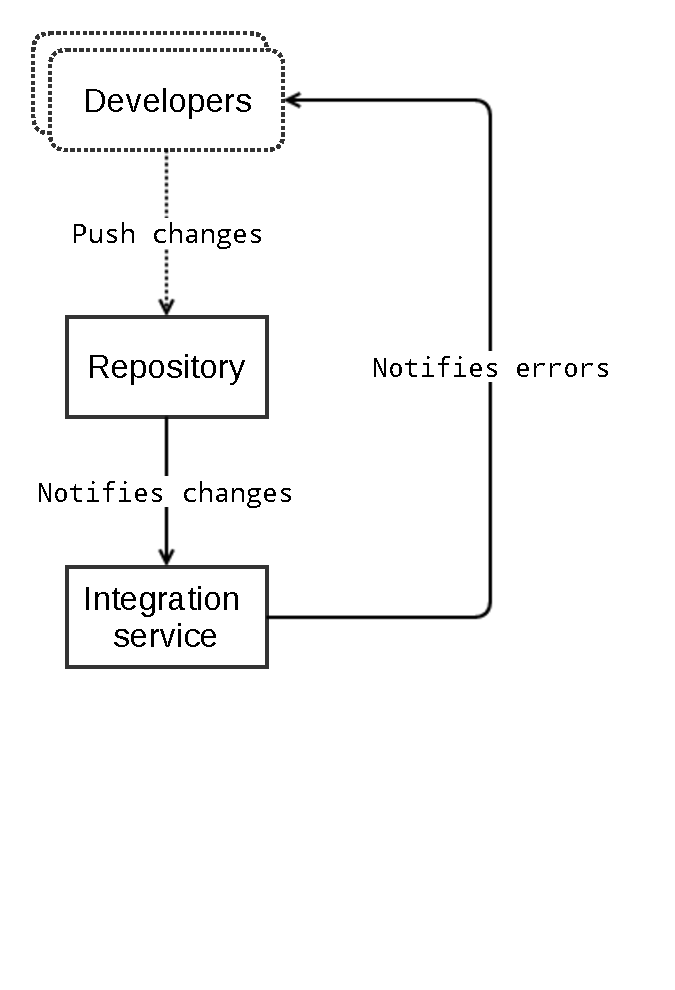
\includegraphics{graphs/ci_errors.pdf}
}
\end{center}
\end{frame}
\begin{frame}{Continuous integration}
\begin{center}
\noindent\resizebox{!}{180pt}{
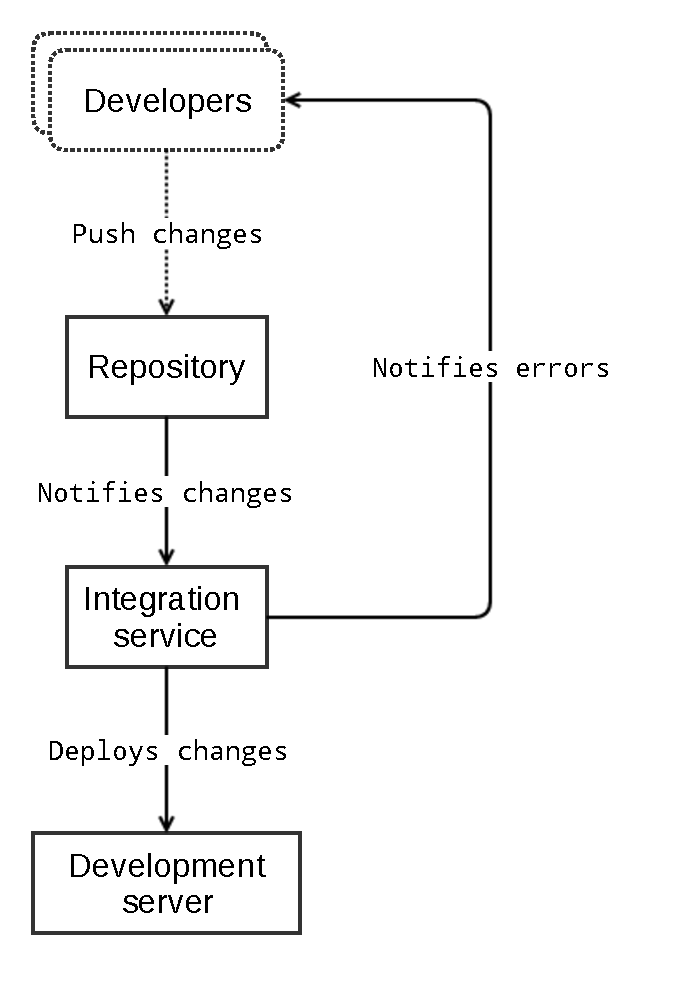
\includegraphics{graphs/ci.pdf}
}
\end{center}
\end{frame}
\subsection{The first prototype}
\begin{frame}{A simple prototype}
\begin{description}
\item[Engine:]
Running one simple player and notifying actions to subscribers.
\item[\texttt{API}:]
Subscribed to the engine and notifying actions to clients.
\item[Client:]
Subscribed to the \texttt{API} and drawing player actions in a web-browser.
\end{description}
\end{frame}
\begin{frame}{The engine architecture}
\begin{figure}[H]
\begin{center}
\noindent\resizebox{\textwidth}{!}{
\begin{tikzpicture}[->,>=stealth',shorten >=1pt,auto,node distance=0.8cm,
    main node/.style={thick,circle,draw,minimum width=2.5cm}]

    \node[main node] (1) {master};

	\node[auto=false] (2) [below=of 1]{\ldots};
    \node[auto=false] (21) [left=of 2]{};
    \node[auto=false] (23) [left=of 21]{};
    \node[auto=false] (22) [right=of 2]{};
    \node[auto=false] (24) [right=of 22]{};

    \node[main node] (3) [left=of 23]{worker$_1$};
    \node[main node] (4) [right=of 24]{worker$_N$};

    \node[auto=false] (5) [below=of 3]{\ldots};
    \node[main node] (6) [left=of 5]{player$_{1,1}$};
    \node[main node] (7) [right=of 5]{player$_{1,{M_1}}$};

    \node[auto=false] (8) [below=of 4]{\ldots};
    \node[main node] (9) [left=of 8]{player$_{N,1}$};
    \node[main node] (10) [right=of 8]{player$_{N,{M_N}}$};


    \path (1) edge (3);
    \path (1) edge (4);

    \path (3) edge (6);
    \path (3) edge (7);

    \path (4) edge (9);
    \path (4) edge (10);
\end{tikzpicture}

}
\end{center}
\caption{Hierarchy of engine processes with $N$ workers and $\sum_{i=1}^N M_i$ players}
\label{engine_arch}
\end{figure}
\end{frame}
\begin{frame}{The prototype result}
\begin{figure}[H]
\begin{center}
\noindent\resizebox{!}{15em}{
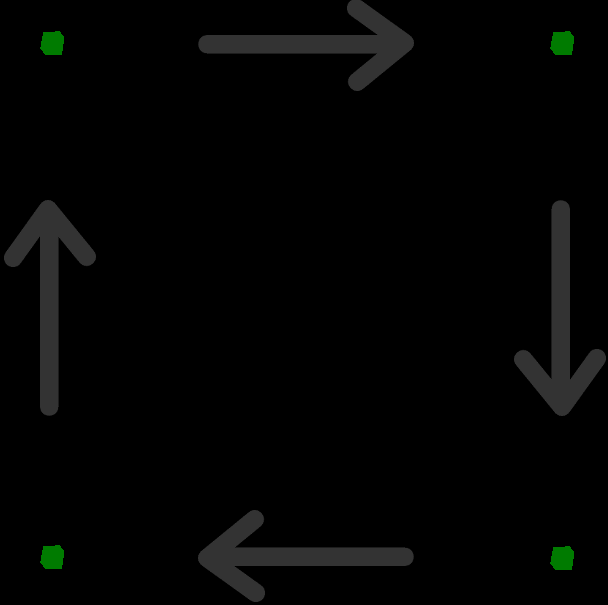
\includegraphics{images/cube_movement.png}
}
\end{center}
\caption{A cube that was moved by the player program}
\label{cube_movement}
\end{figure}
\end{frame}
\subsection{Continuous integration}
\begin{frame}{Continuous integration stack}
\begin{center}
\noindent\resizebox{!}{180pt}{
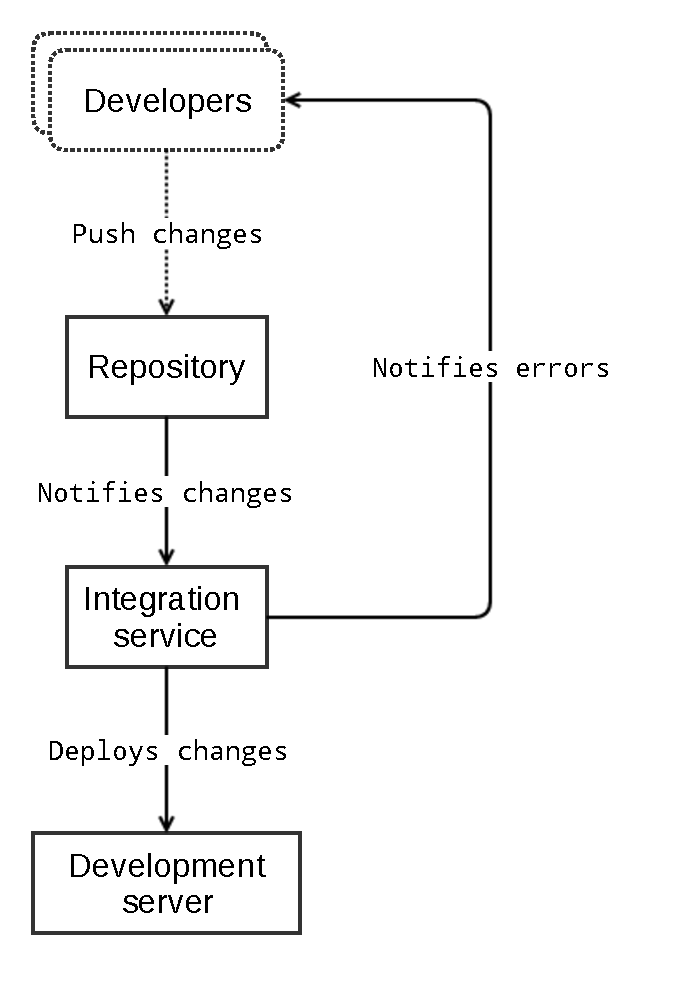
\includegraphics{graphs/ci.pdf}
}
\end{center}
\end{frame}
\begin{frame}{Continuous integration stack}
\begin{center}
\noindent\resizebox{!}{180pt}{
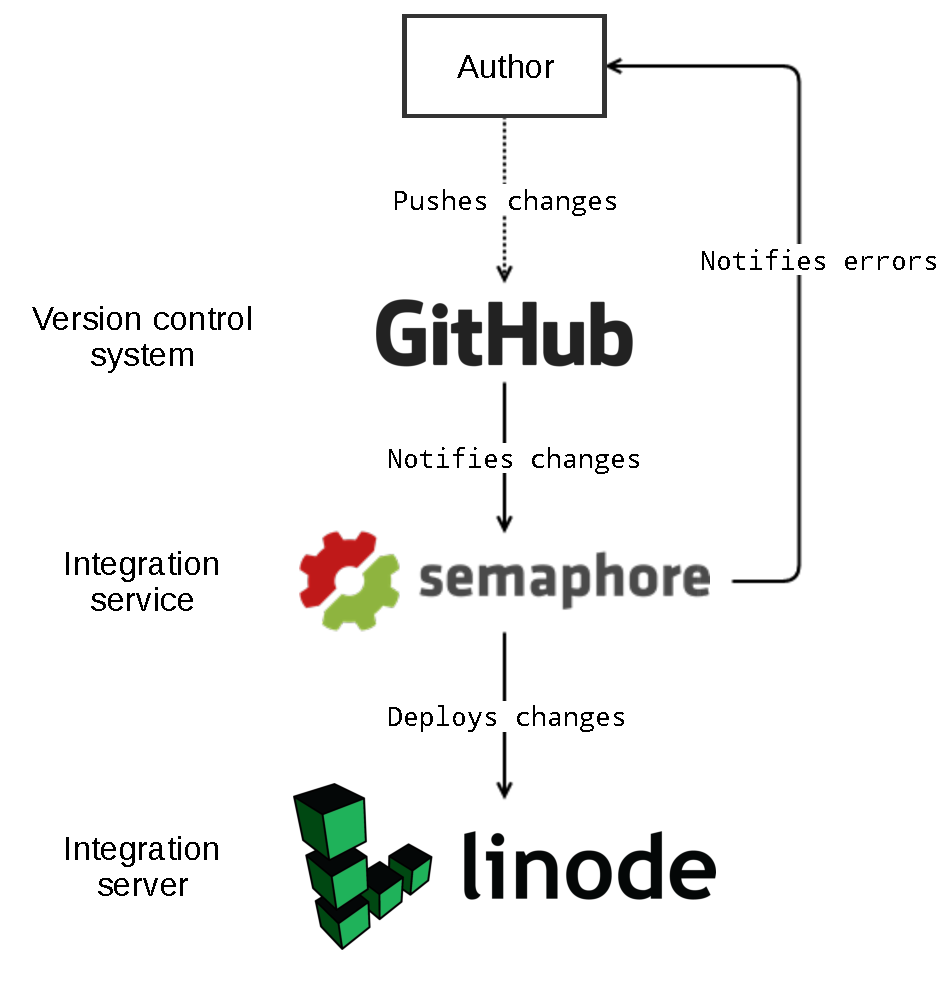
\includegraphics{graphs/ci_final.pdf}
}
\end{center}
\end{frame}
\subsection{The log system}
\begin{frame}{Match replay}
\begin{center}
An \texttt{MMPG} match might last weeks.
      $$\Downarrow$$
      Players will miss parts of the match.
      $$\Downarrow$$
      Players need to be able to replay the past of the match.
\end{center}
\end{frame}
\begin{frame}{Event sourcing}
\makebox[\textwidth]{
\noindent\resizebox{!}{180pt}{
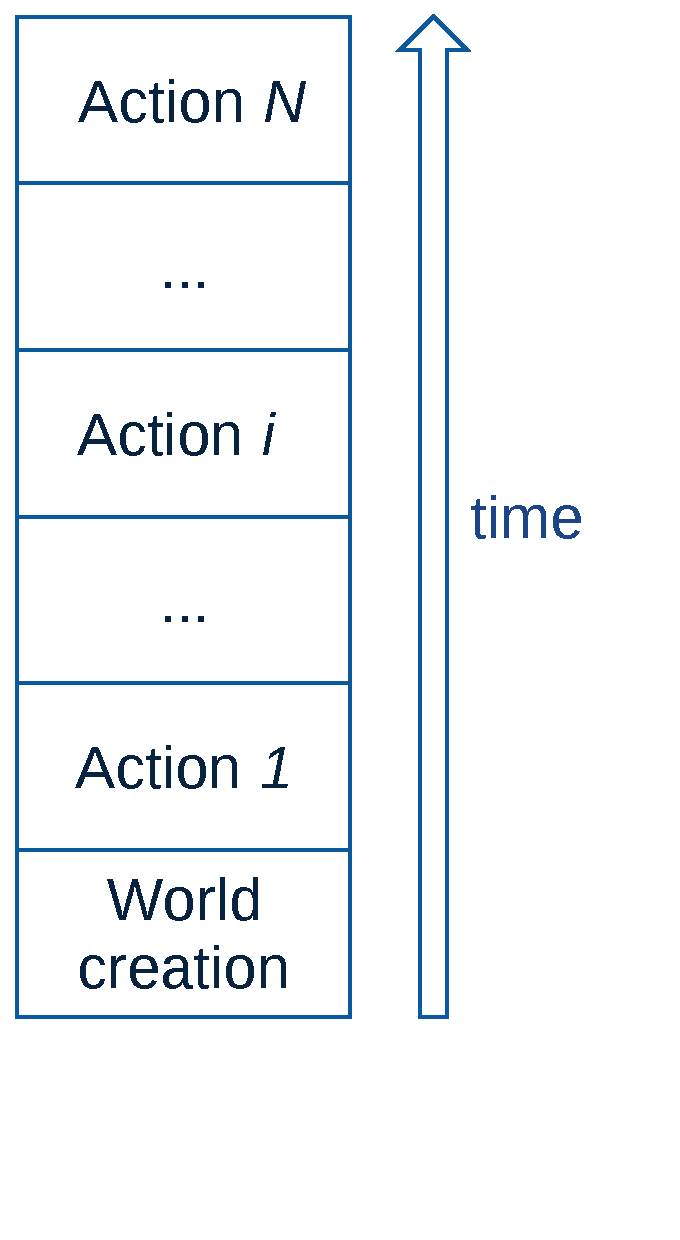
\includegraphics{graphs/eventsourcing.pdf}
}
}
\end{frame}
\begin{frame}{Snapshots}
\makebox[\textwidth]{
\noindent\resizebox{!}{180pt}{
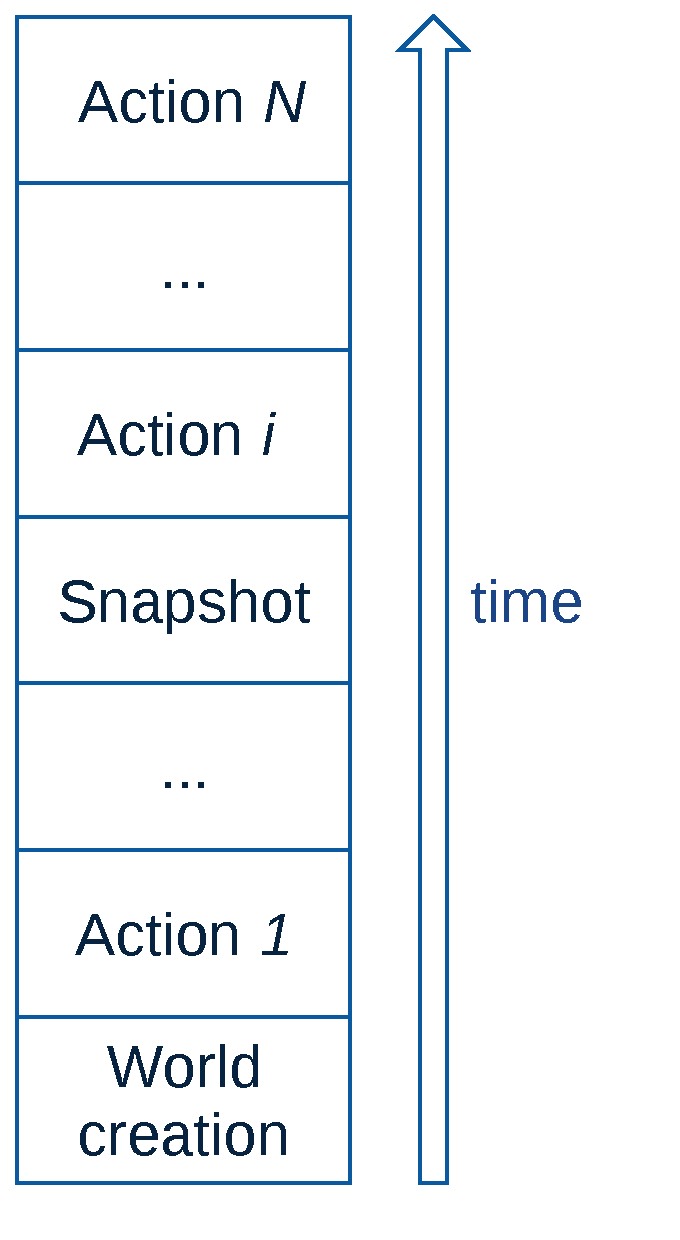
\includegraphics{graphs/eventsourcing_snapshot.pdf}
}
}
\end{frame}
\begin{frame}{Log files}
\makebox[\textwidth]{
\noindent\resizebox{!}{150pt}{
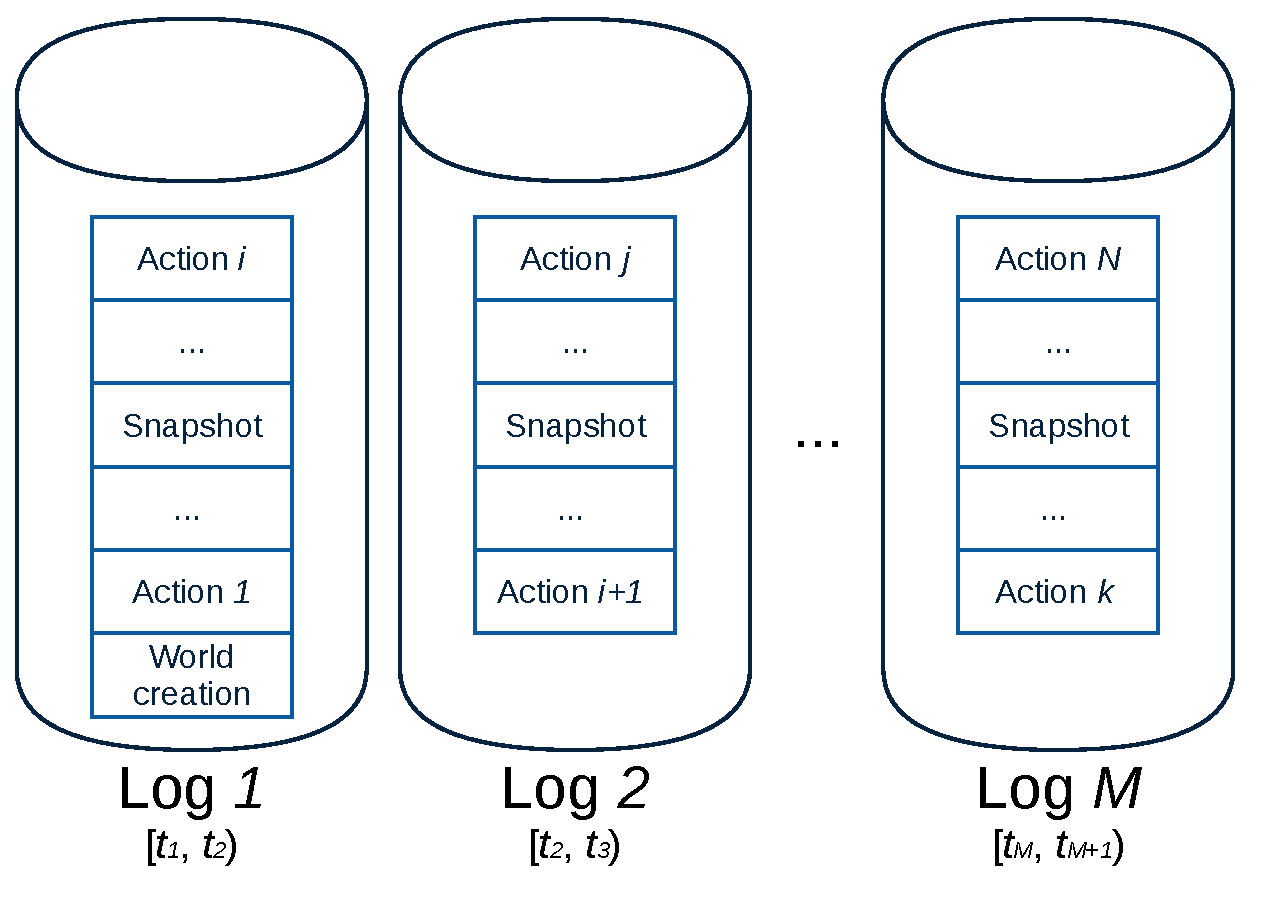
\includegraphics{graphs/log_files.pdf}
}
}
$$t_2 - t_1 = t_3 - t_2 = \cdots = t_{M+1} - t_M = \text{log interval}$$
\end{frame}
\subsection{Deployment of AI}
\begin{frame}{Authentication}
\begin{figure}[H]
\makebox[\textwidth]{
\noindent\resizebox{!}{180pt}{

\includegraphics{images/login_ok.png}
}
\noindent\resizebox{!}{180pt}{

\includegraphics{images/login_error.png}
}
}
\caption{Login form. Valid (left). Invalid (right)}
\end{figure}
\end{frame}
\begin{frame}{\texttt{AI} hot-swapping}
\begin{figure}[H]
\makebox[\textwidth]{
\noindent\resizebox{!}{180pt}{
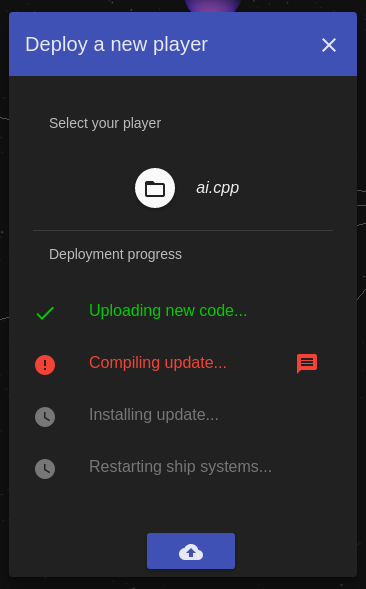
\includegraphics{images/deploy_error.png}
}
}
\caption{Player deployment with a compilation error}
\end{figure}
\end{frame}
\subsection{The first world}
\begin{frame}{Galcon}
\begin{figure}[H]
\noindent\resizebox{!}{180pt}{
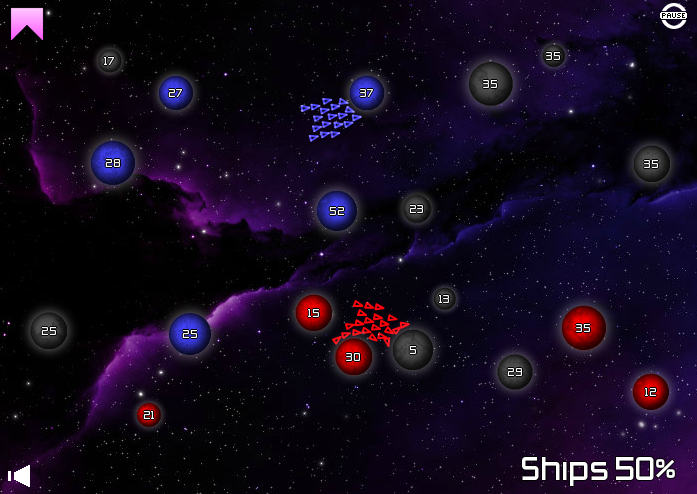
\includegraphics{images/galcon.png}
}
\caption{Galcon 2}
\end{figure}
\end{frame}
\begin{frame}{Planetary system approximation}
\begin{figure}[H]
\begin{minipage}{.65\textwidth}
\noindent\resizebox{\textwidth}{!}{
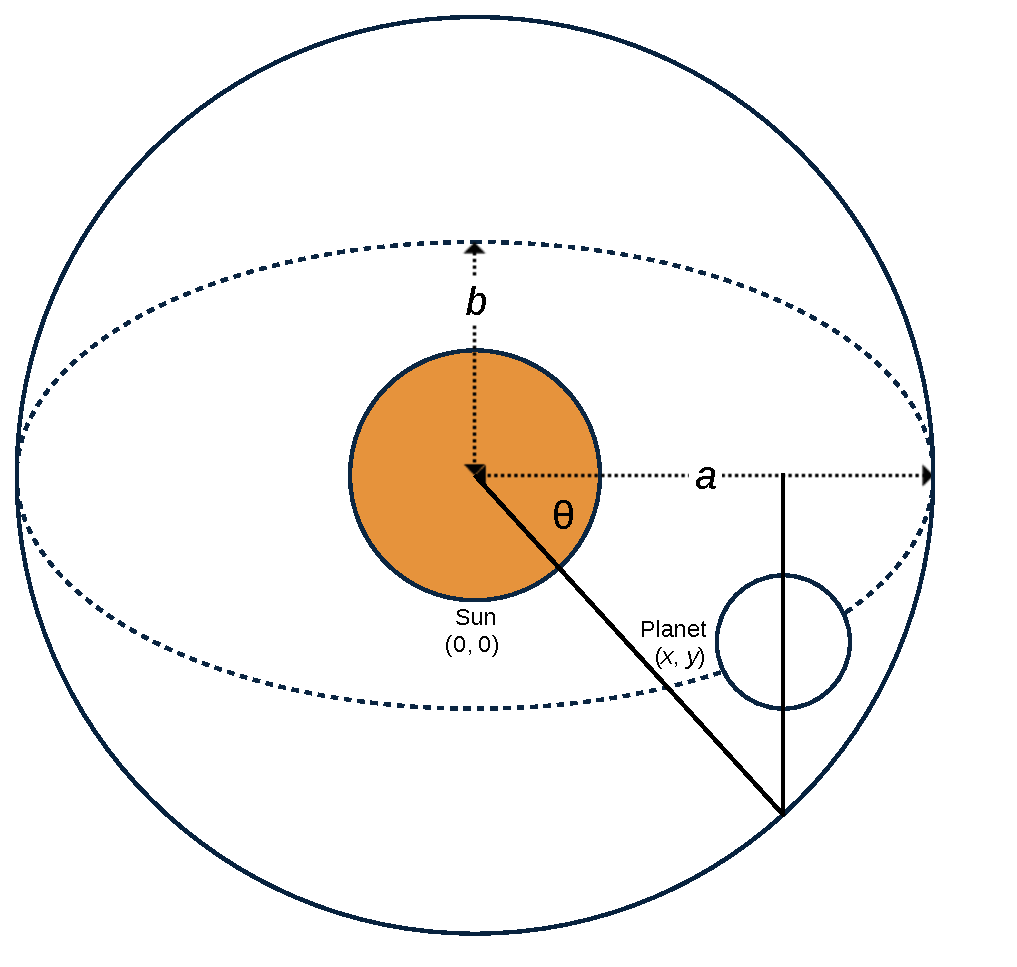
\includegraphics{graphs/planet_position.pdf}
}
\end{minipage}
\begin{minipage}{.3\textwidth}
$$x = a \: cos(\theta)$$
           $$y = b \: sin(\theta)$$
\end{minipage}
\end{figure}
\end{frame}
\begin{frame}{Procedural generation of planetary systems}
\begin{center}
\noindent\resizebox{!}{180pt}{
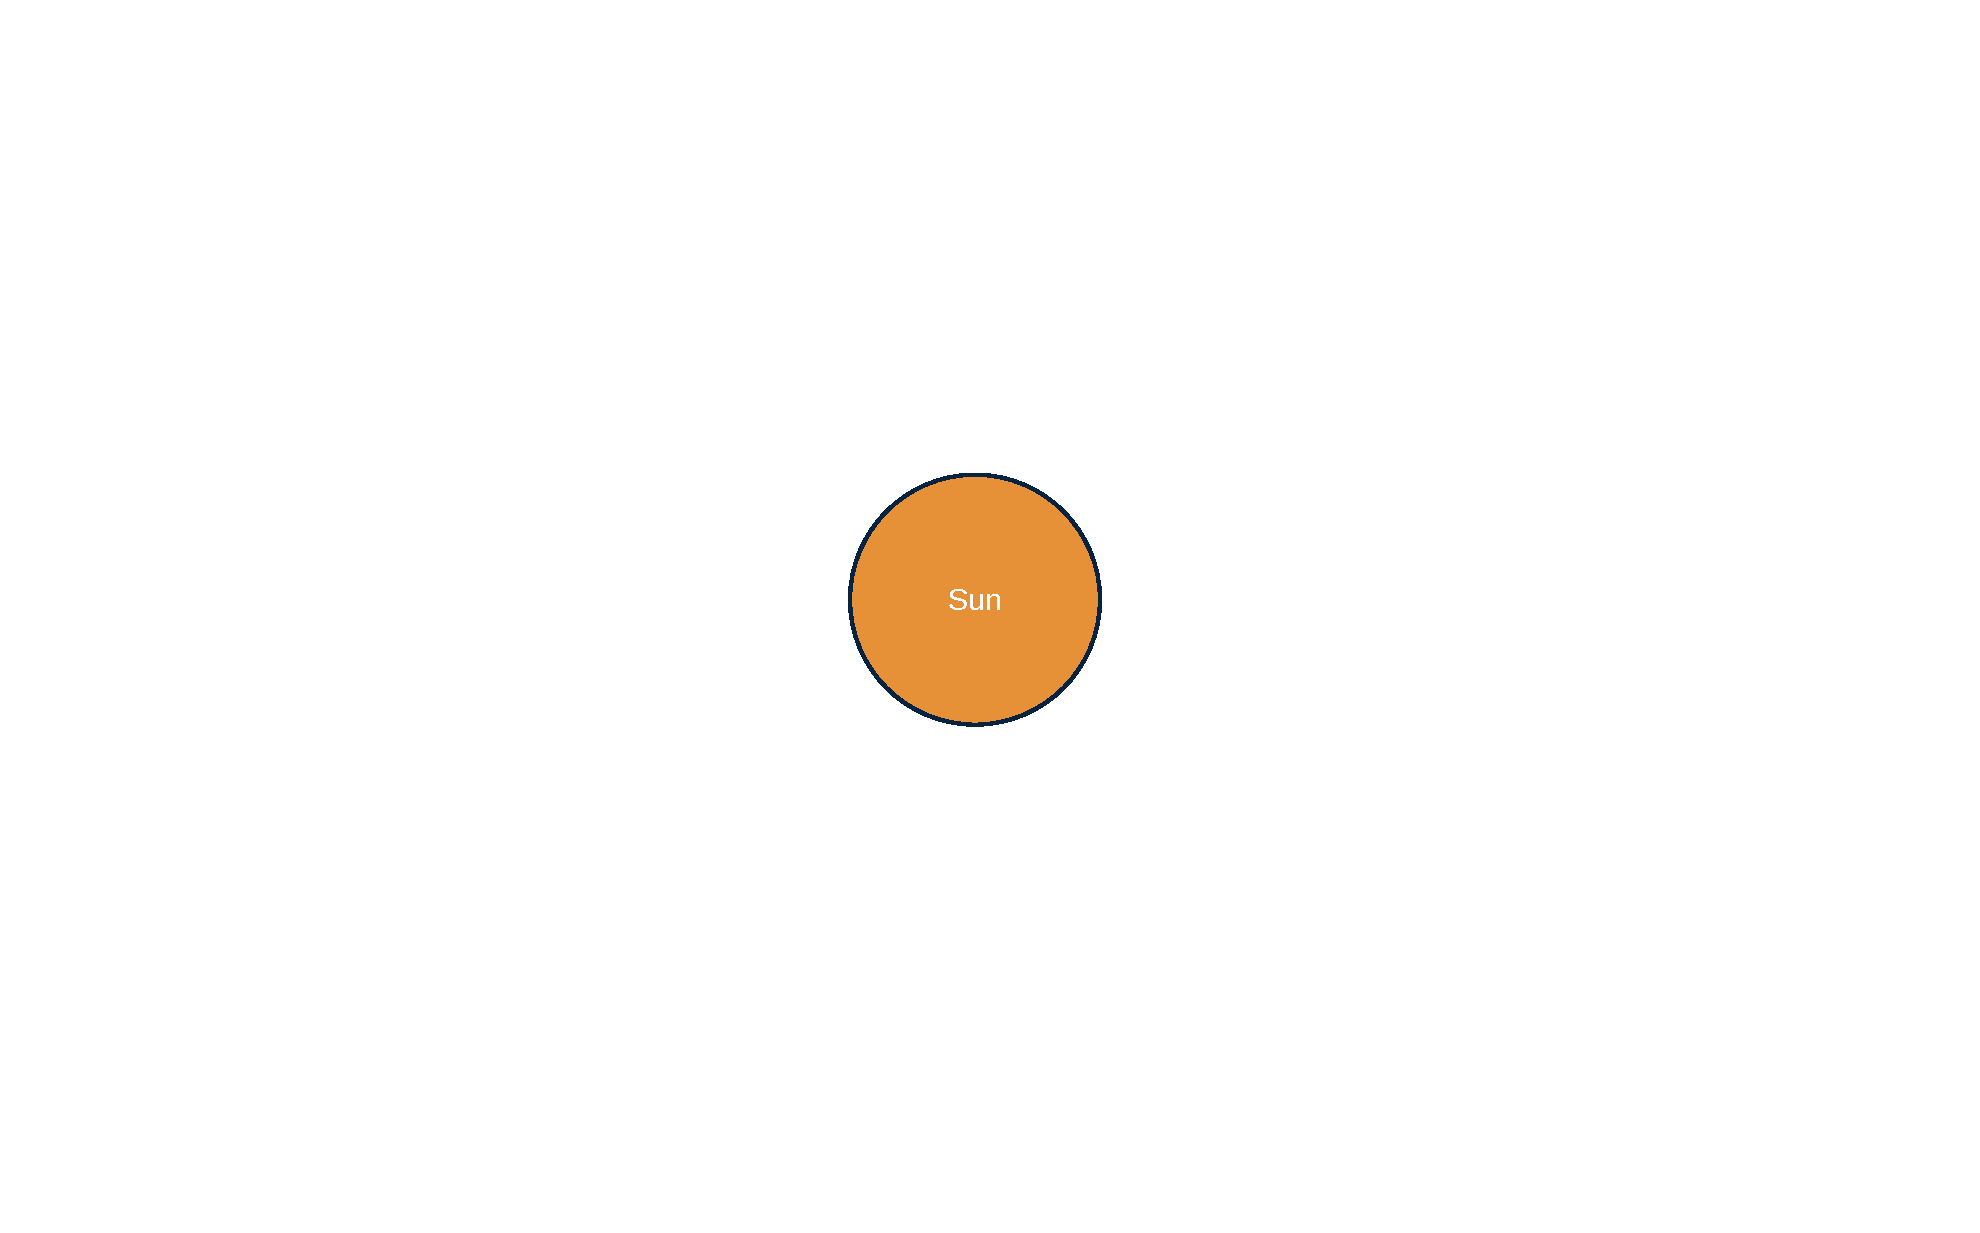
\includegraphics{graphs/generation_initial.pdf}
}
\end{center}
\end{frame}
\begin{frame}{Procedural generation of planetary systems}
\begin{center}
\noindent\resizebox{!}{180pt}{
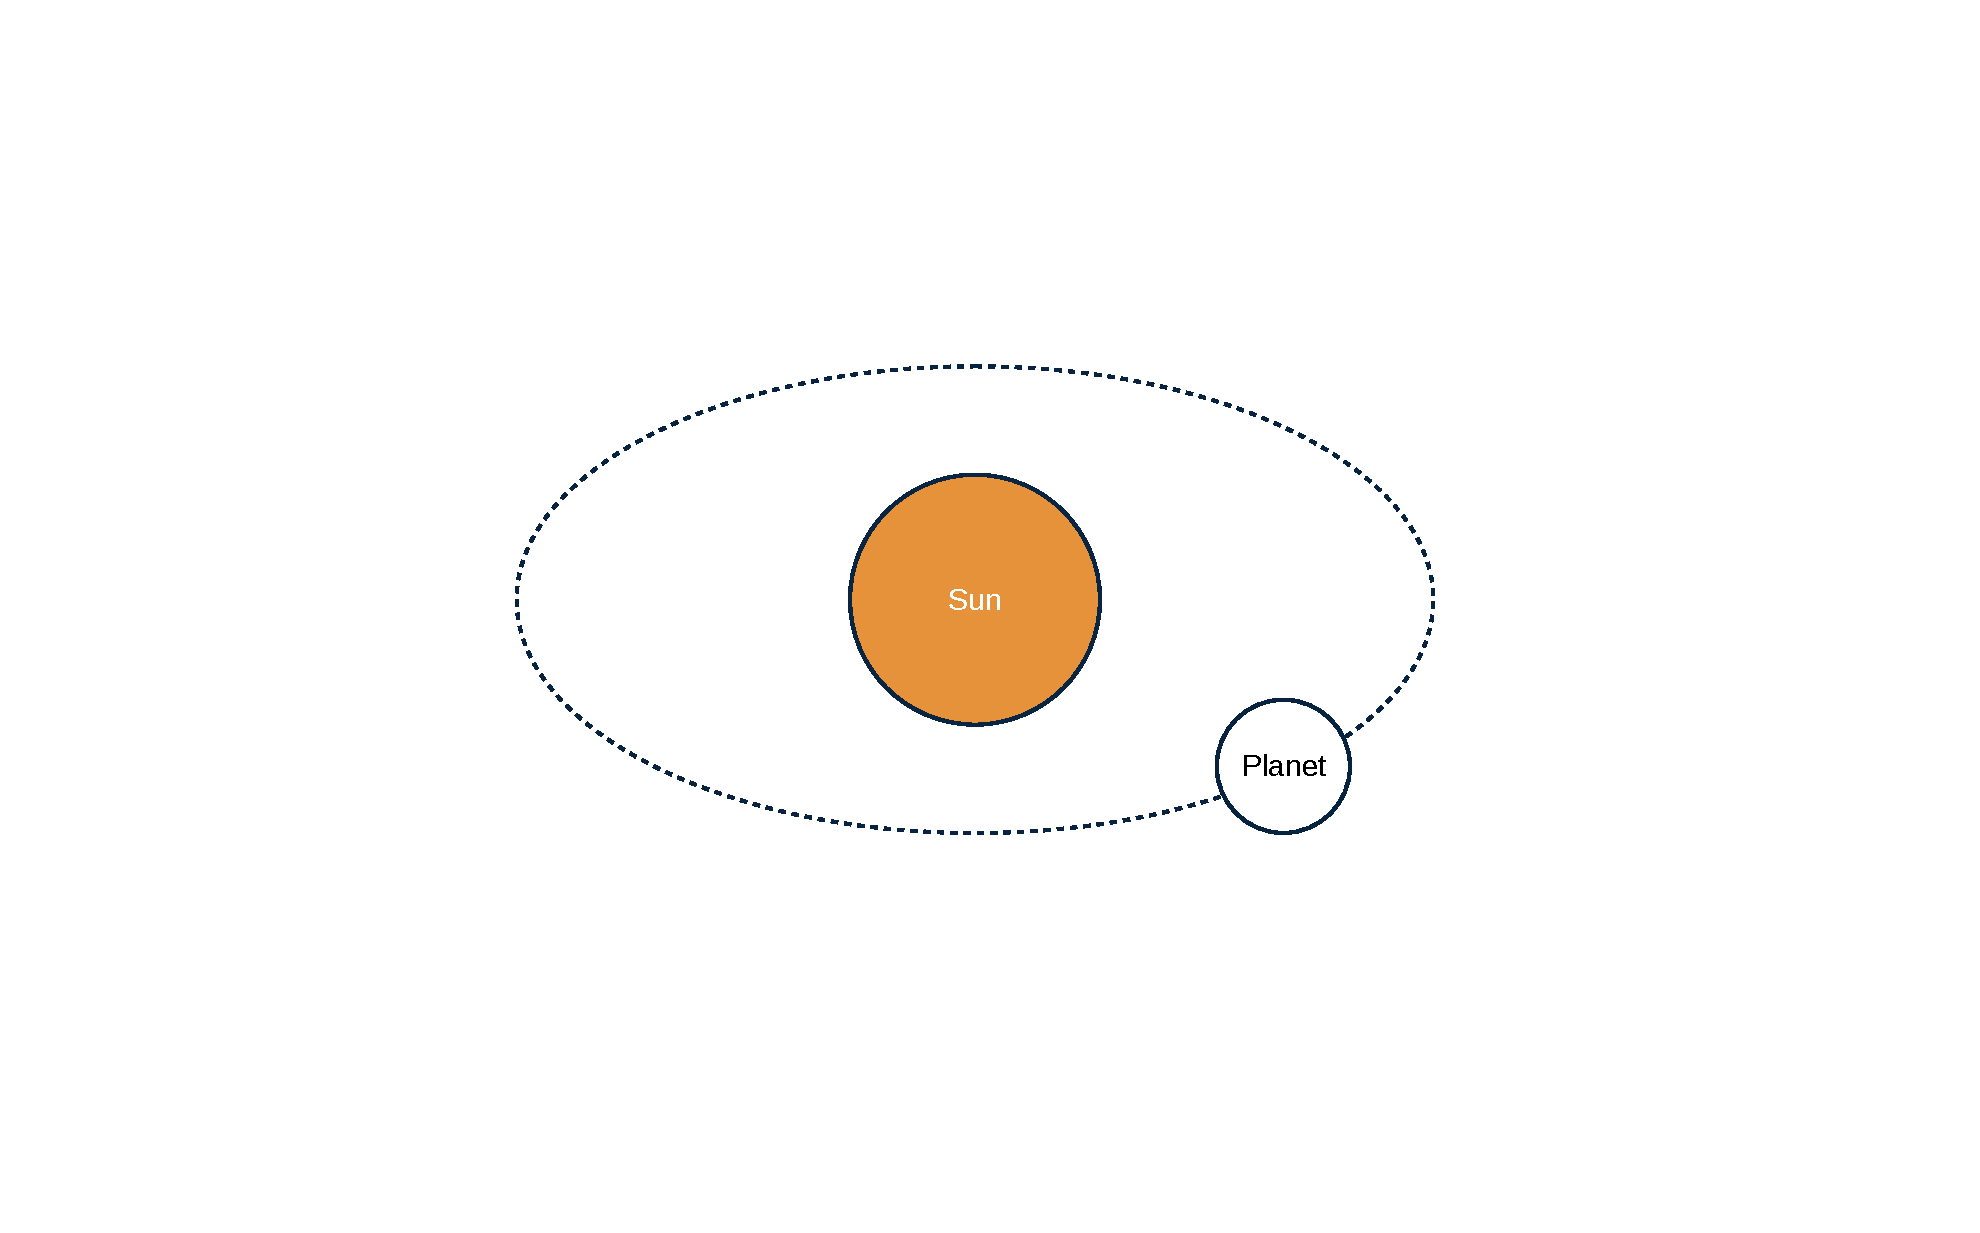
\includegraphics{graphs/generation_planet1.pdf}
}
\end{center}
\end{frame}
\begin{frame}{Procedural generation of planetary systems}
\begin{center}
\noindent\resizebox{!}{180pt}{
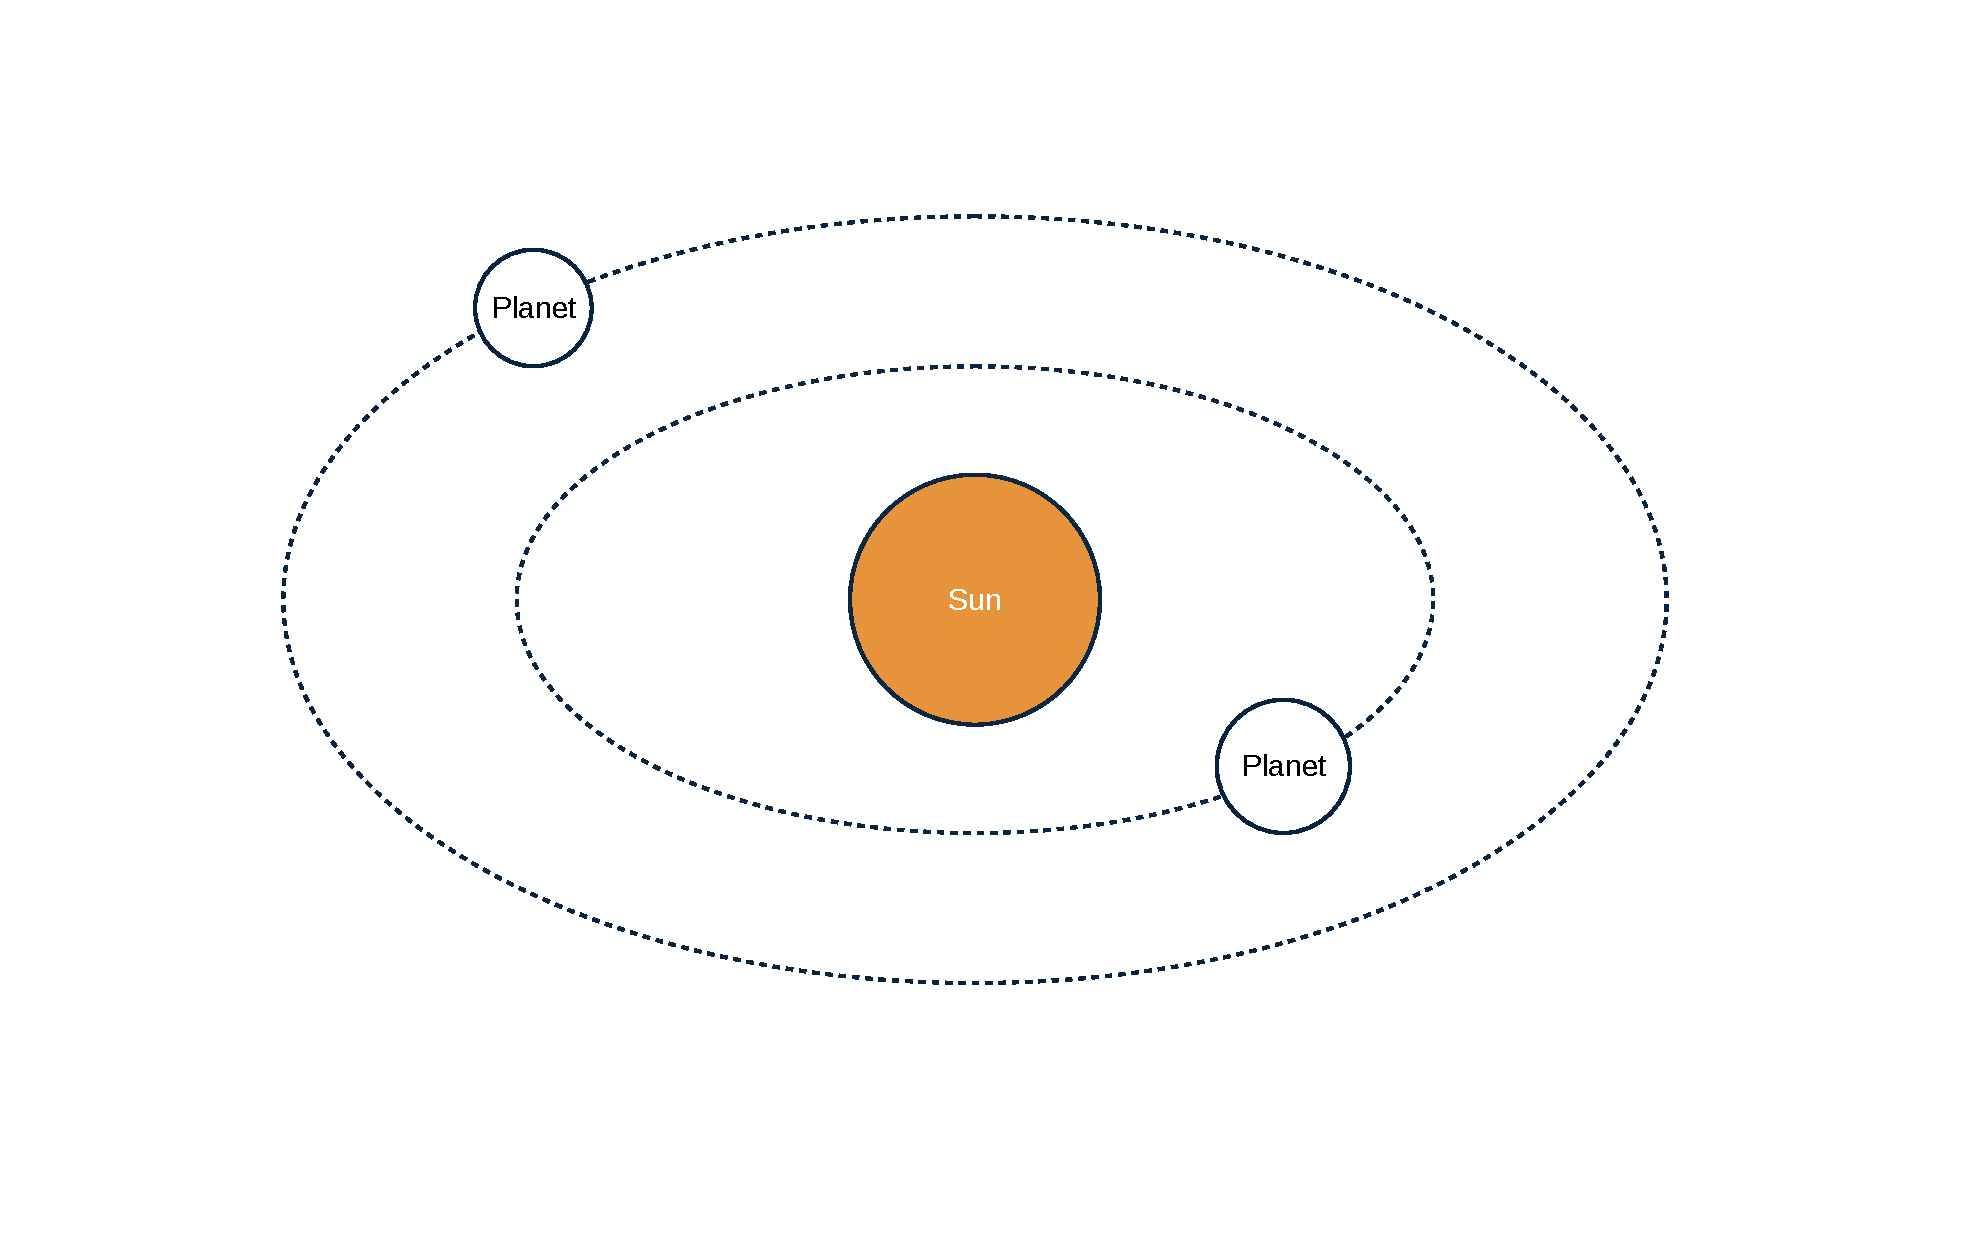
\includegraphics{graphs/generation_planet2.pdf}
}
\end{center}
\end{frame}
\begin{frame}{Procedural generation of planetary systems}
\begin{center}
\noindent\resizebox{!}{180pt}{
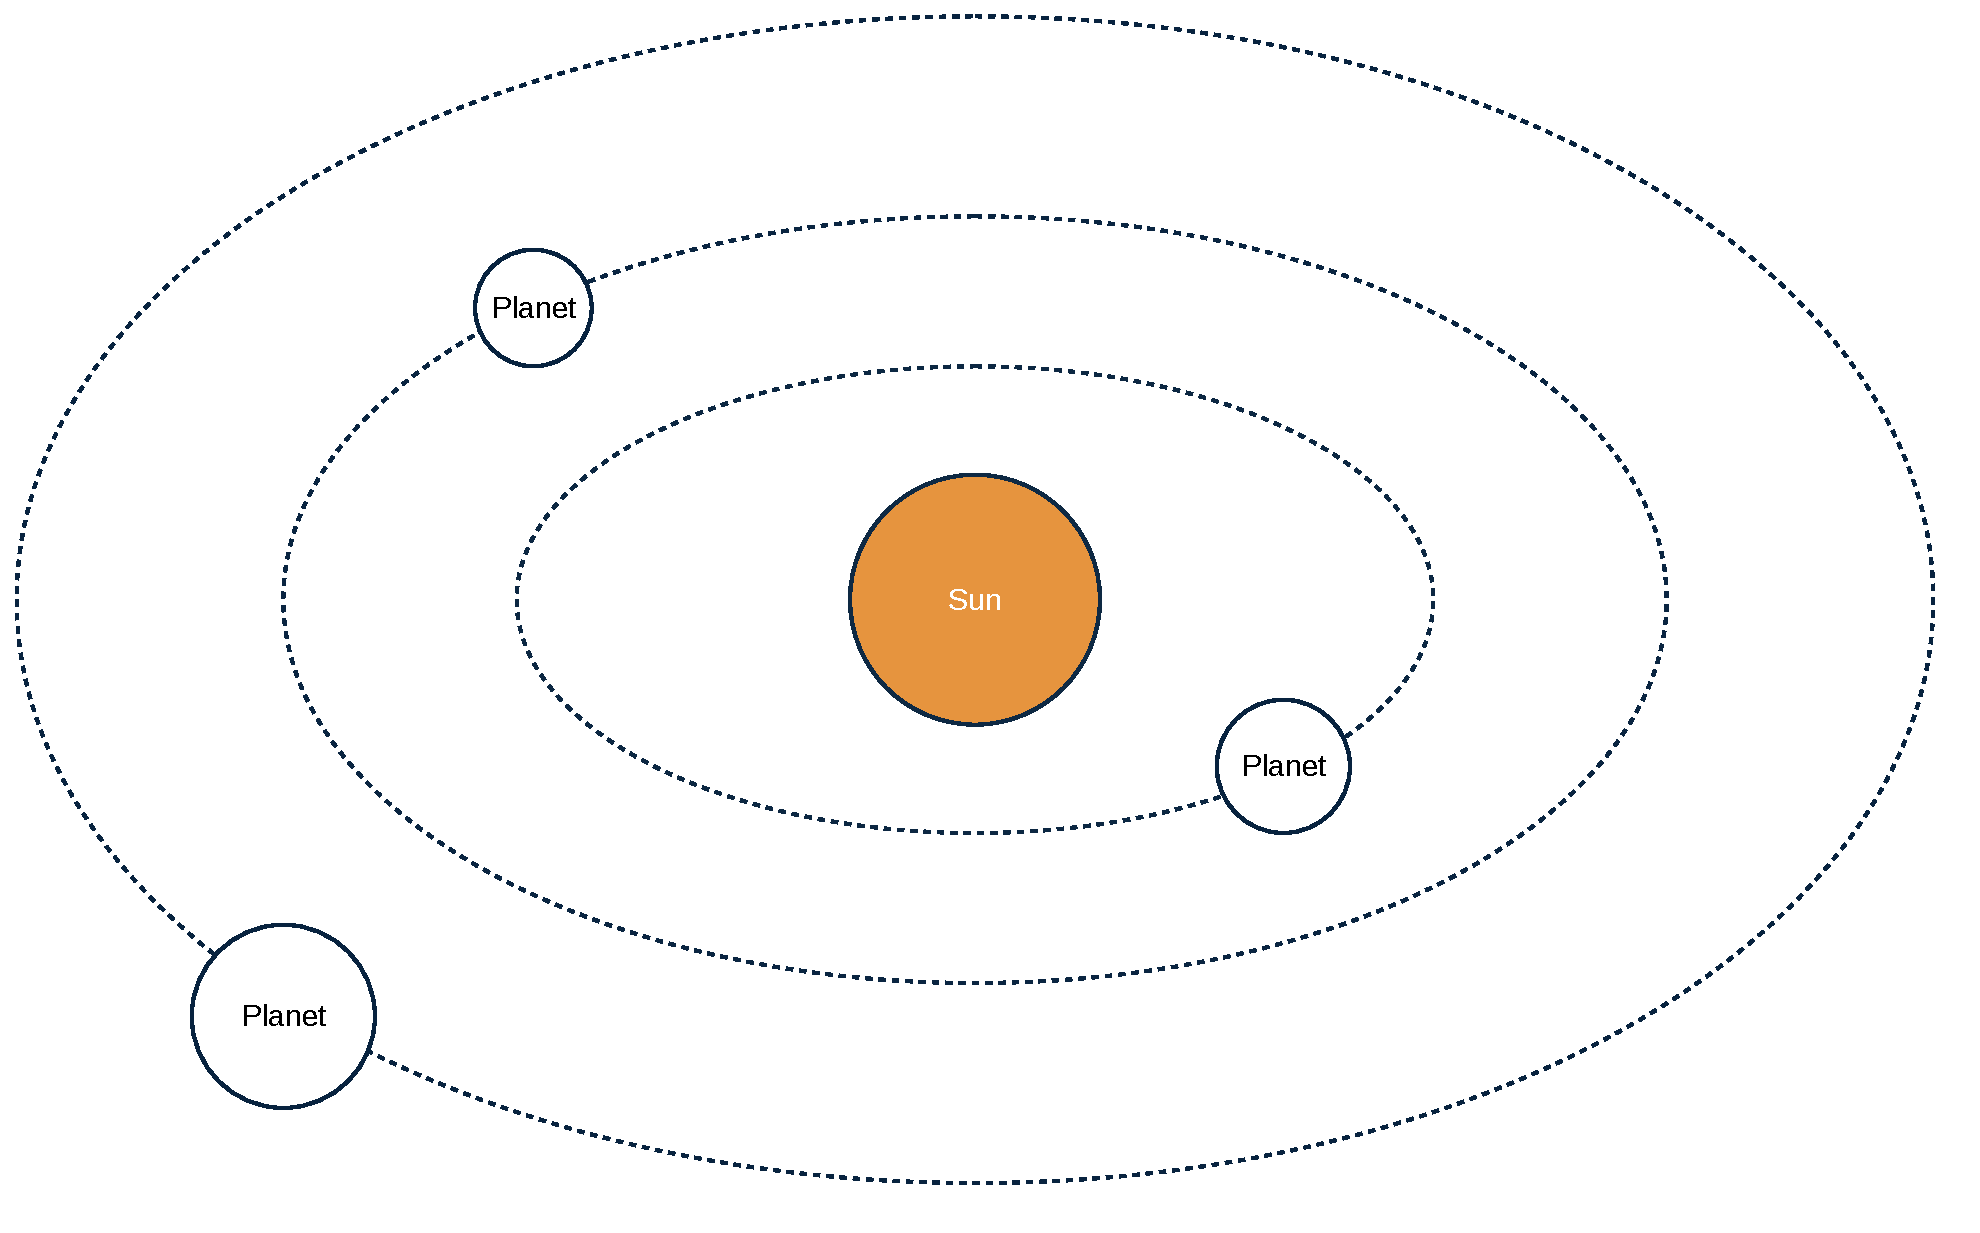
\includegraphics{graphs/generation_planets.pdf}
}
\end{center}
\end{frame}
\begin{frame}{Procedural generation of planetary systems}
\begin{center}
\noindent\resizebox{!}{180pt}{
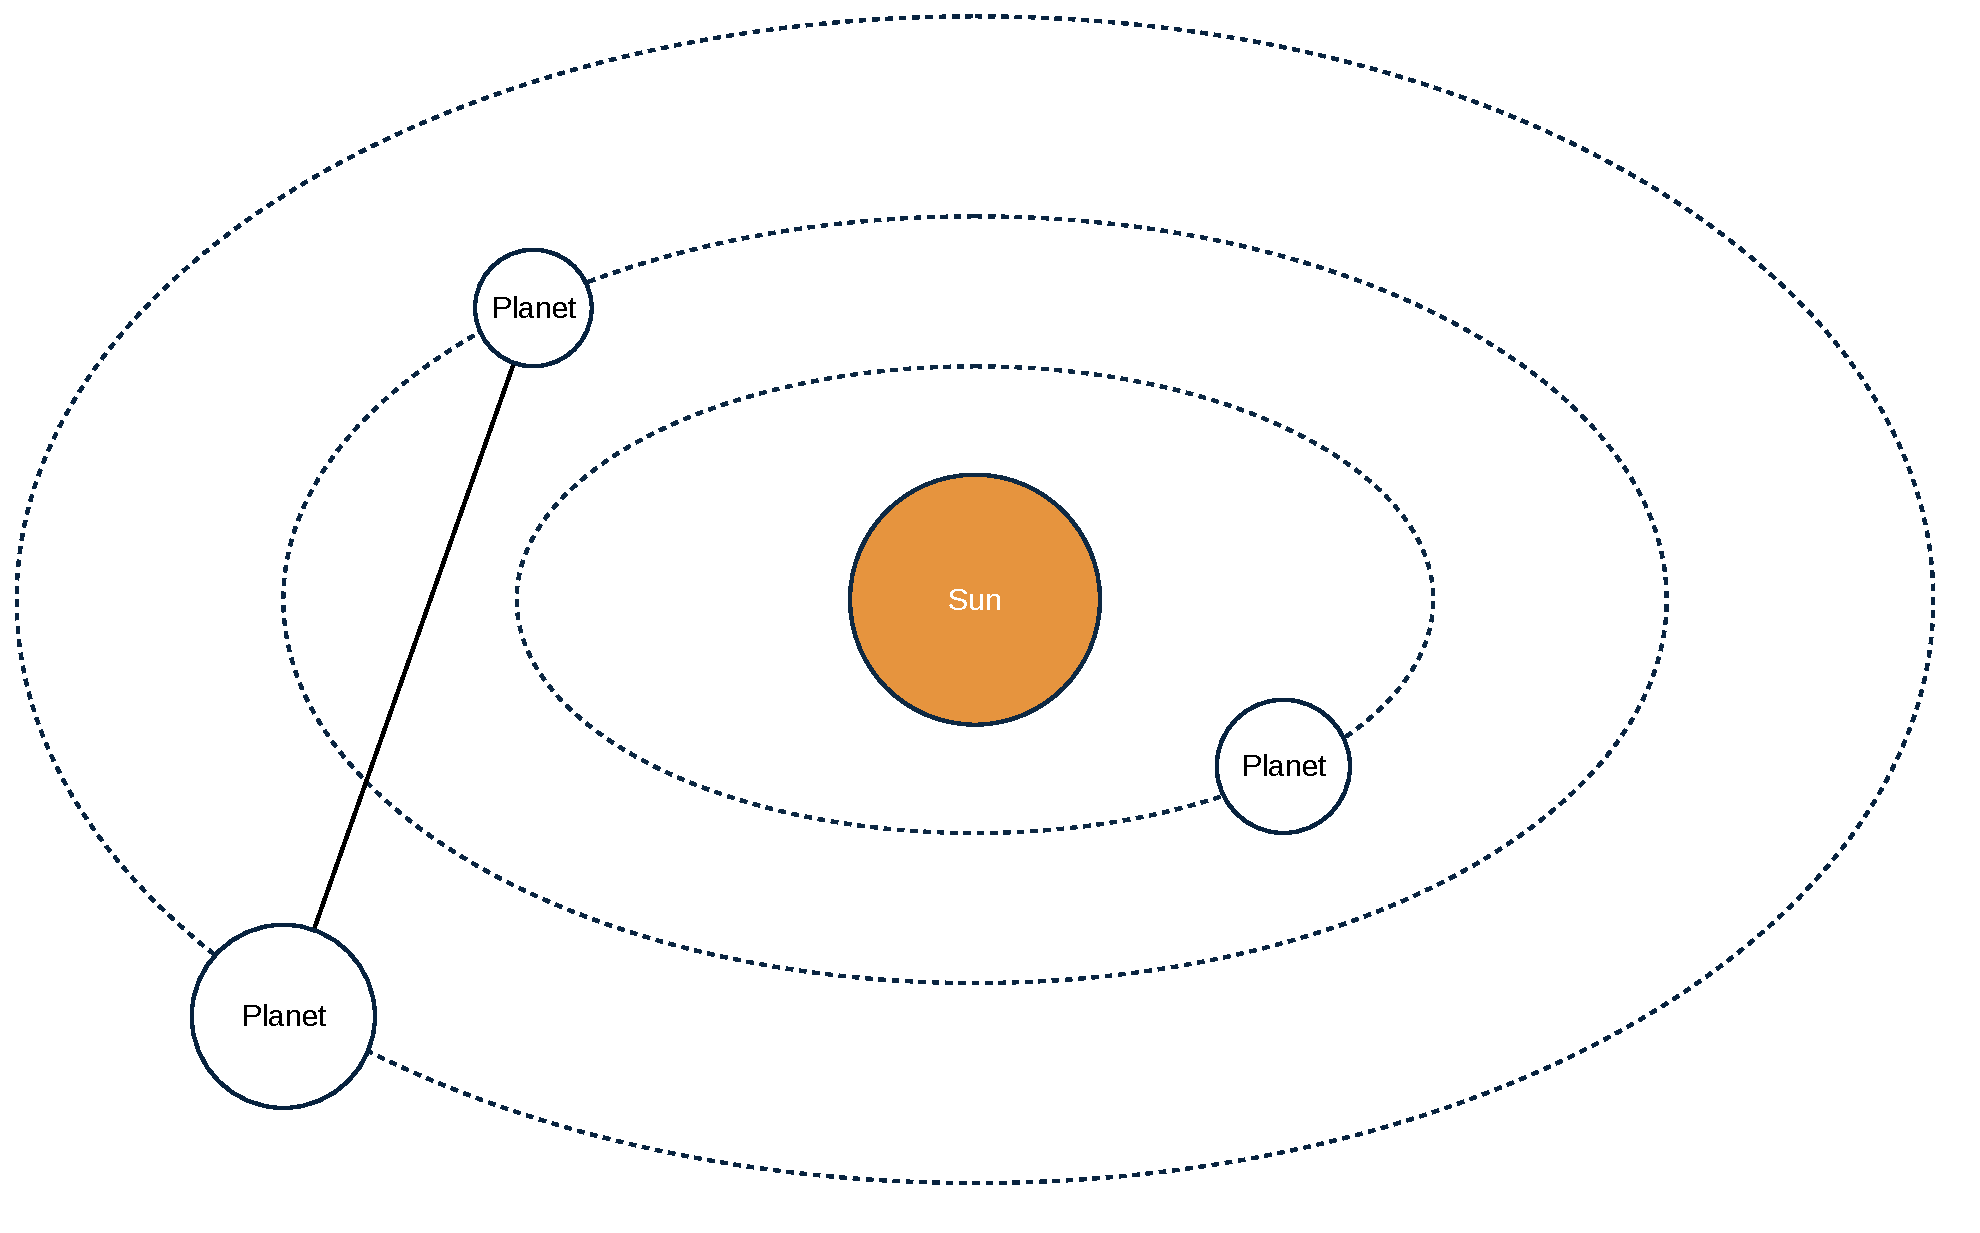
\includegraphics{graphs/generation_connection.pdf}
}
\end{center}
\end{frame}
\begin{frame}{Procedural generation of planetary systems}
\begin{center}
\noindent\resizebox{!}{180pt}{
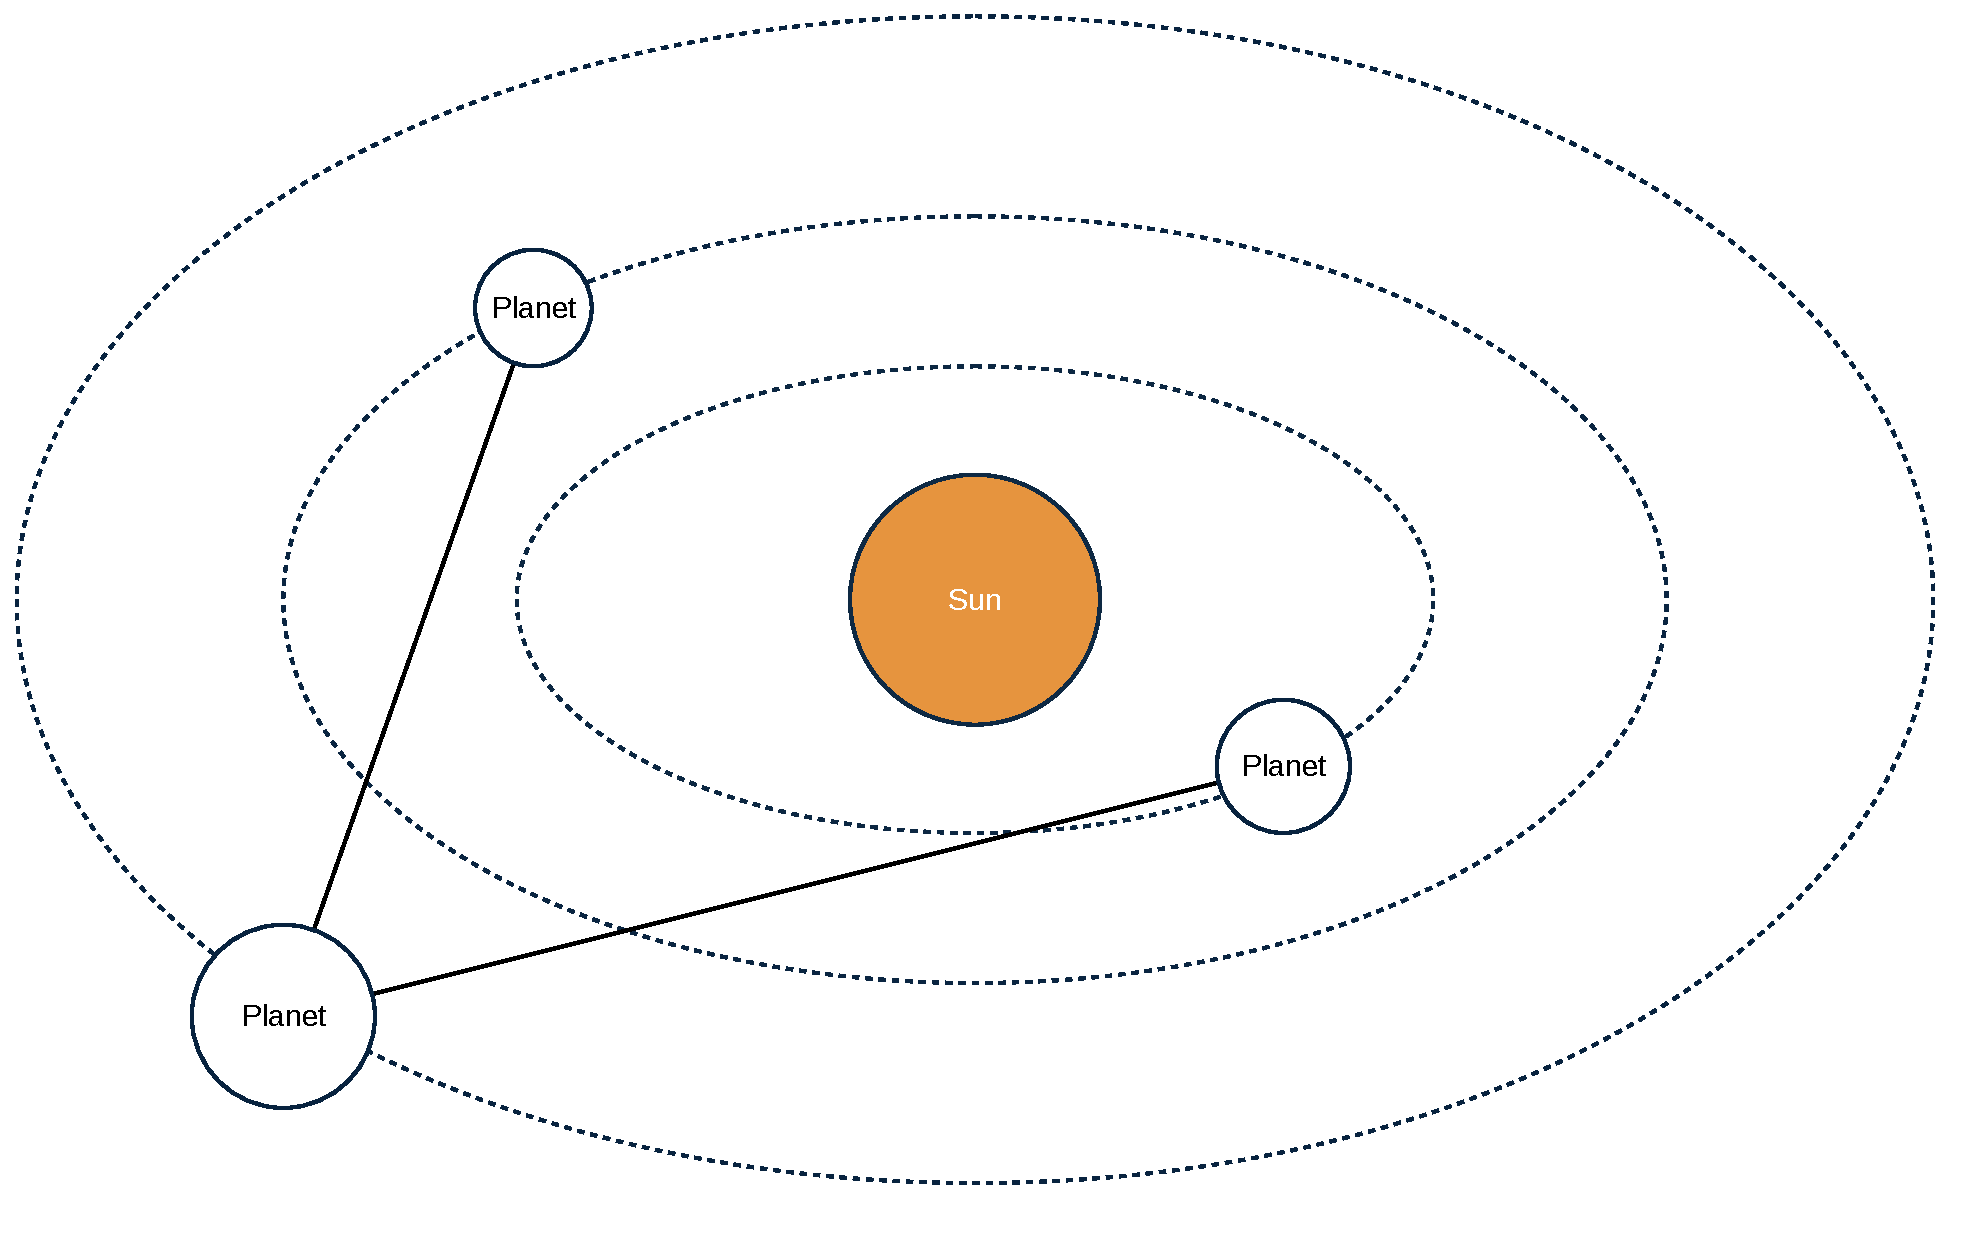
\includegraphics{graphs/generation.pdf}
}
\end{center}
\end{frame}
\subsection{A whole galaxy}
\begin{frame}{Connecting systems}
\begin{center}
\noindent\resizebox{!}{180pt}{
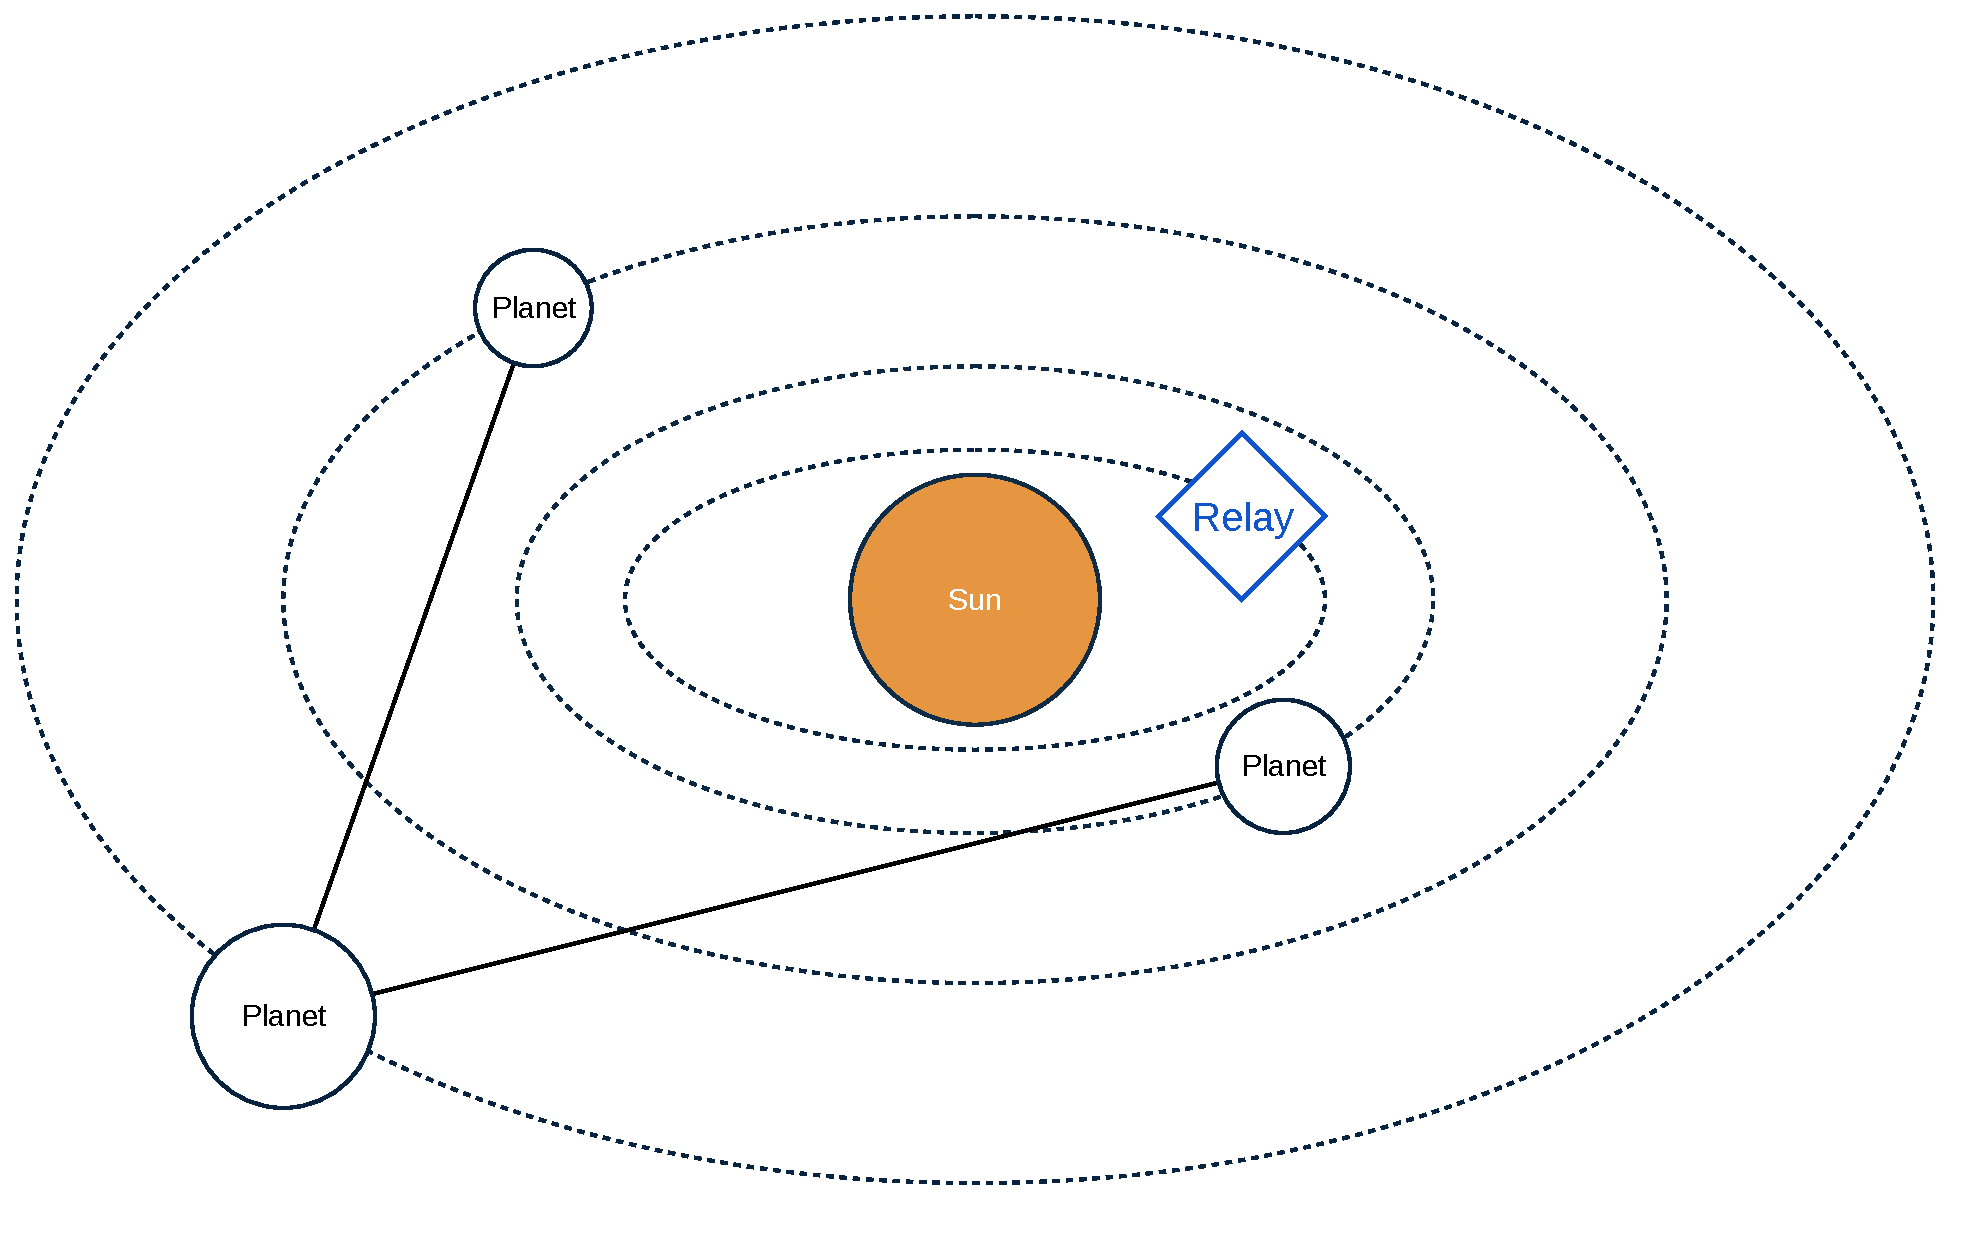
\includegraphics{graphs/relay_planets.pdf}
}
\end{center}
\end{frame}
\begin{frame}{Connecting systems}
\begin{center}
\noindent\resizebox{!}{180pt}{
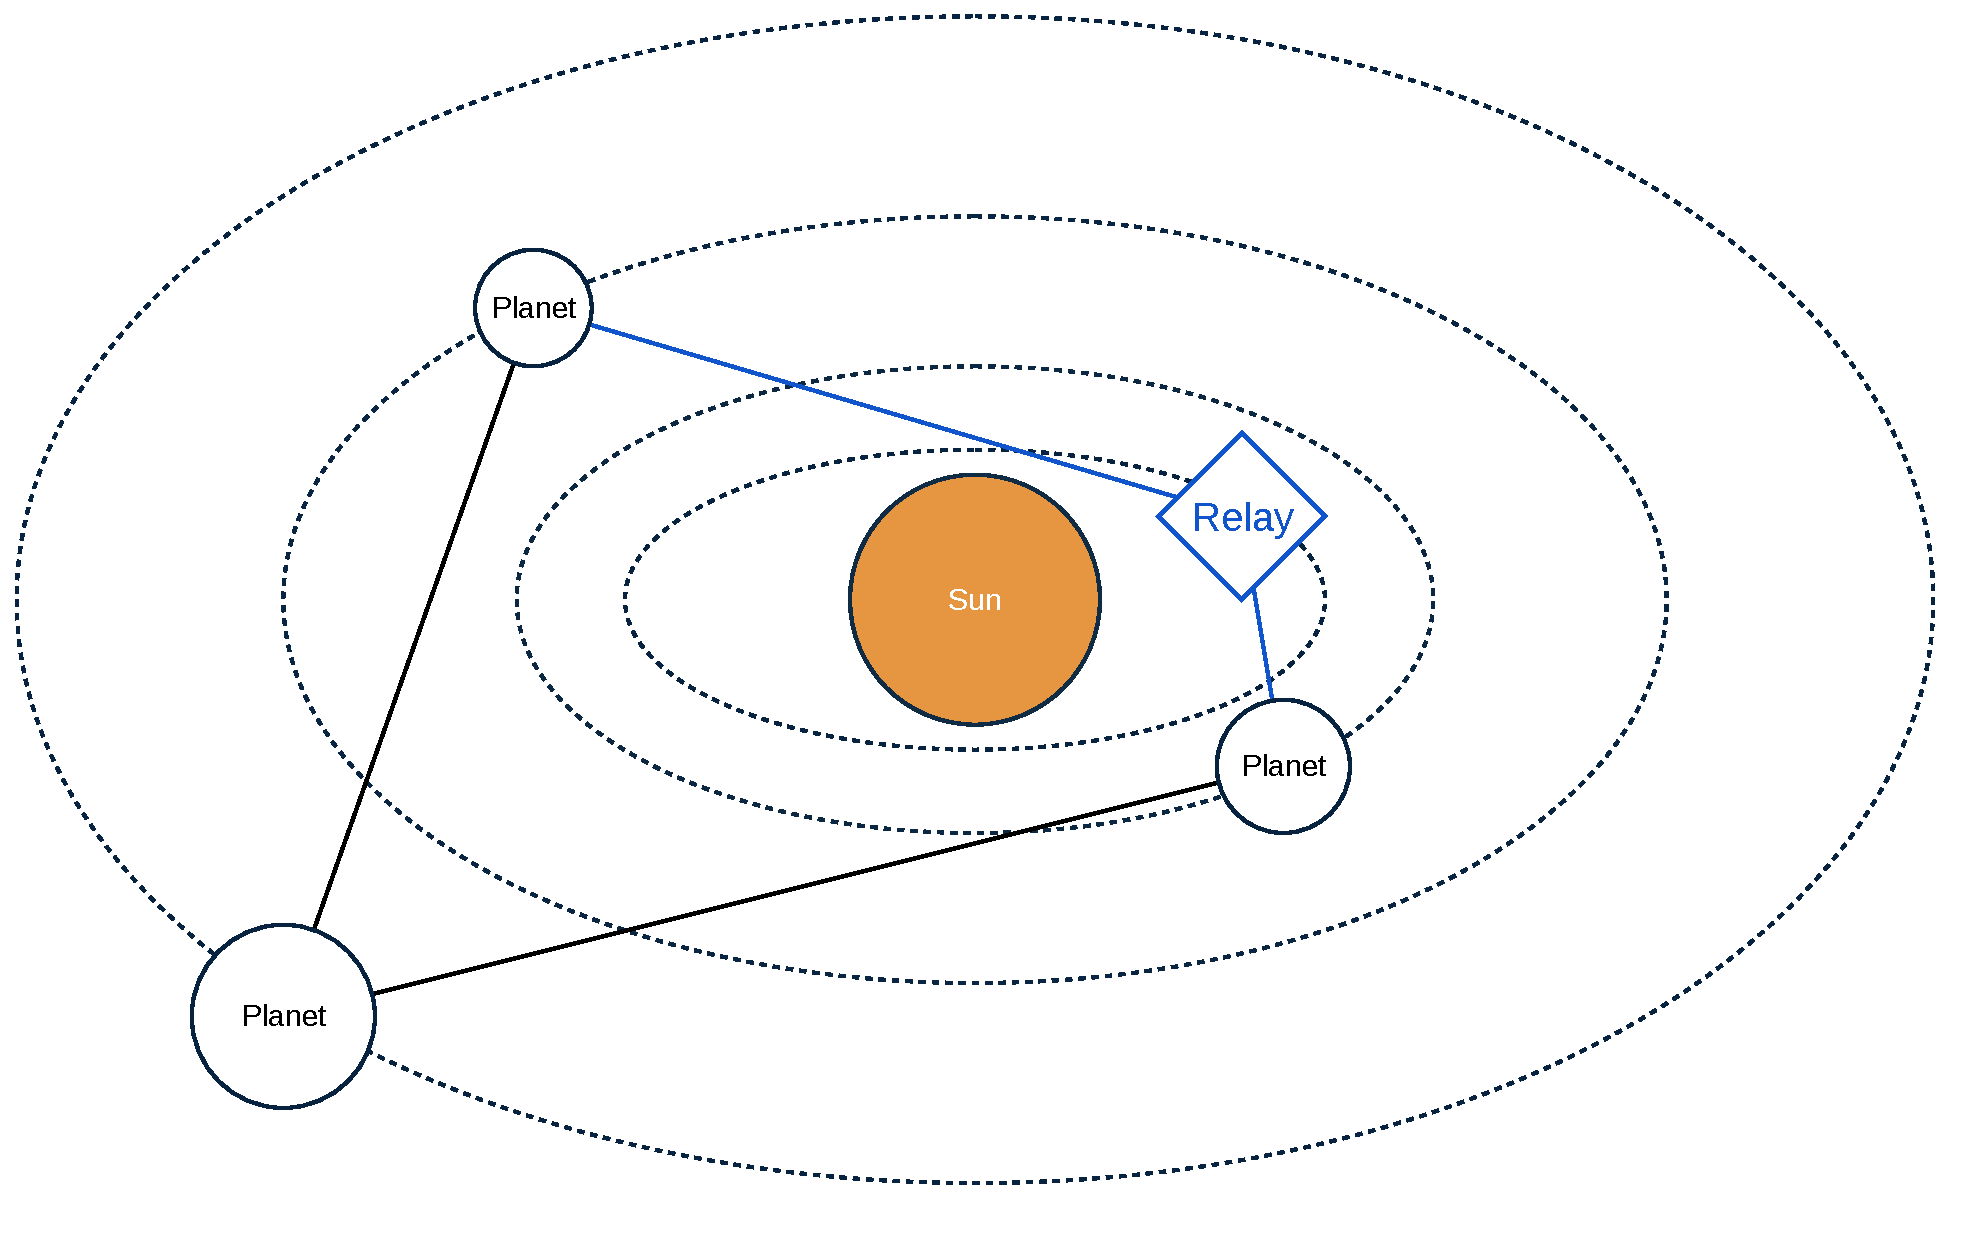
\includegraphics{graphs/relay.pdf}
}
\end{center}
\end{frame}
\begin{frame}{Generating multiple systems}
\begin{center}
300 planetary systems
      $$\Downarrow$$
      CPU usage increase from 2\% to 20\% in the Linode
\end{center}
\end{frame}
\begin{frame}[fragile]{Separating world structure from dynamic data}
\begin{figure}[H]
\begin{center}
\inputminted[fontsize=\tiny]{js}{code/snapshot.json}
\end{center}
\caption{A snapshot before the optimization}
\end{figure}
\end{frame}
\begin{frame}{Separating world structure from dynamic data}
\begin{figure}[H]
\begin{center}
\inputminted{js}{code/optimized_snapshot.json}
\end{center}
\caption{A snapshot after the optimization}
\end{figure}
\end{frame}
\begin{frame}{Separating world structure from dynamic data}
\begin{figure}[H]
\noindent\resizebox{\textwidth}{!}{
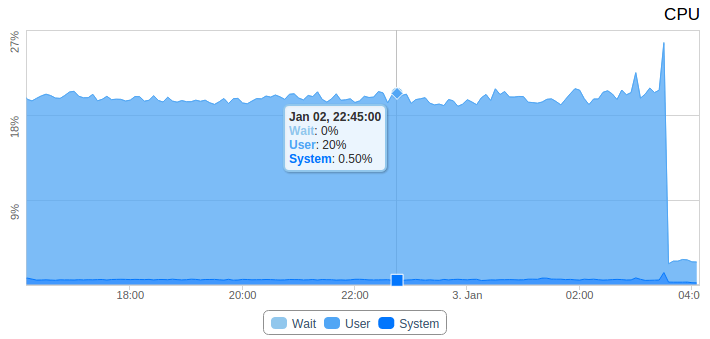
\includegraphics{images/cpu_galaxy.png}
}
\caption{CPU usage drop after separating world structure from dynamic data}
\end{figure}
\end{frame}
\begin{frame}{Rendering a galaxy}
\begin{minipage}{.60\textwidth}
\noindent\resizebox{\textwidth}{!}{

\includegraphics{images/galaxy_50_players.png}
}
\end{minipage}
\begin{minipage}{.35\textwidth}
$$x(t) = at \: cos(t + \theta)$$
         $$y(t) = at \: sin(t + \theta)$$
\end{minipage}
\end{frame}
\begin{frame}{Rendering a galaxy}
\begin{figure}[H]
\noindent\resizebox{\textwidth}{!}{

\includegraphics{images/identicons.png}
}
\caption{Identicons}
\end{figure}
\end{frame}
\begin{frame}{Rendering a galaxy}
\begin{center}
\noindent\resizebox{!}{180pt}{
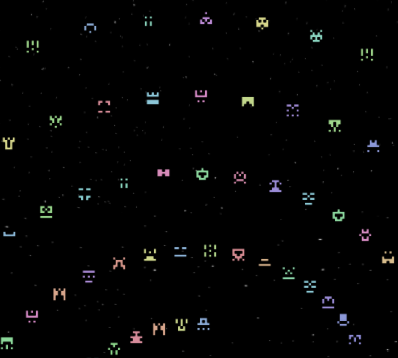
\includegraphics{images/galaxy_identicons.png}
}
\end{center}
\end{frame}
\section{Demonstration}
\subsection{Live}
\begin{frame}{Space Wars}
\begin{center}
\emph{Live demo}
\end{center}
\end{frame}
\section{Evaluation}
\subsection{Validation}
\begin{frame}{Validation of secondary objectives}
\begin{enumerate}
\item
Develop an abstract game engine
\item
Allow hot-swapping of \texttt{AIs}
\item
Implement a real-time webviewer
\item
Make the infrastructure scalable and stable
\item
Create a game example
\end{enumerate}
\end{frame}
\begin{frame}{Validation of secondary objectives}
\begin{enumerate}
\item
Develop an abstract game engine \Checkmark
\item
Allow hot-swapping of \texttt{AIs} \Checkmark
\item
Implement a real-time webviewer \Checkmark
\item
Make the infrastructure scalable and stable
\item
Create a game example \Checkmark
\end{enumerate}
\end{frame}
\begin{frame}{Stability}
\begin{figure}[H]
\noindent\resizebox{\textwidth}{!}{
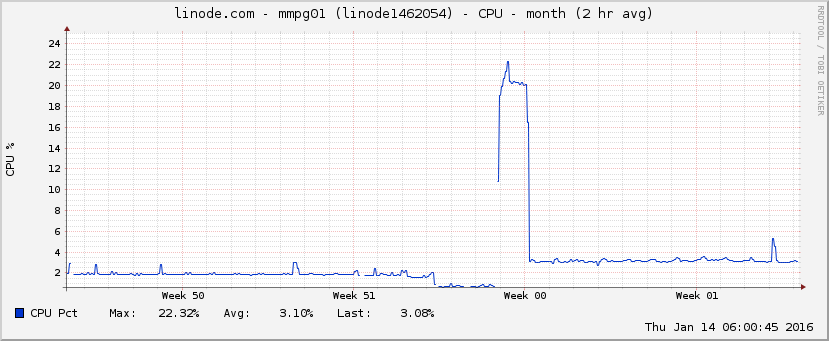
\includegraphics{images/mmpg_cpu.png}
}
\caption{CPU usage of the platform in a 30 day period (Linode 1024)}
\end{figure}
\end{frame}
\begin{frame}{Scalability}
\begin{figure}[H]
\noindent\resizebox{\textwidth}{!}{
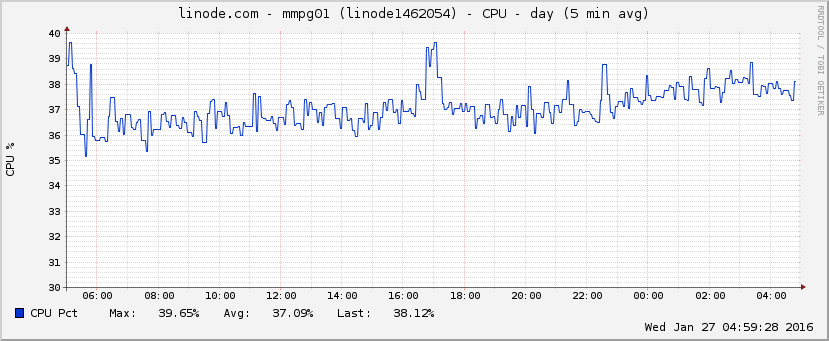
\includegraphics{images/mmpg_cpu_50_players.png}
}
\caption{CPU usage of the platform with 50 players and 300 planetary systems in a day (Linode 1024)}
\end{figure}
\end{frame}
\begin{frame}{Validation of secondary objectives}
\begin{enumerate}
\item
Develop an abstract game engine \Checkmark
\item
Allow hot-swapping of \texttt{AIs} \Checkmark
\item
Implement a real-time webviewer \Checkmark
\item
Make the infrastructure scalable and stable
\item
Create a game example \Checkmark
\end{enumerate}
\end{frame}
\begin{frame}{Validation of secondary objectives}
\begin{enumerate}
\item
Develop an abstract game engine \Checkmark
\item
Allow hot-swapping of \texttt{AIs} \Checkmark
\item
Implement a real-time webviewer \Checkmark
\item
Make the infrastructure scalable and stable \Checkmark
\item
Create a game example \Checkmark
\end{enumerate}
\end{frame}
\begin{frame}{Validation of the main objective}
\emph{Develop a set of components that ease the creation and the usage of \texttt{MMPGs}.}
\begin{itemize}
\item
Abstract game engine \Checkmark
\item
Client library \Checkmark
\item
Documentation \texttimes
\end{itemize}
\end{frame}
\subsection{Time management}
\begin{frame}{Planning timeline}
\begin{figure}[H]
\begin{center}
\noindent\resizebox{!}{180pt}{
\begin{ganttchart}[hgrid, vgrid]{1}{25}
\gantttitle{2015}{20}
\gantttitle{2016}{5}
\\
\gantttitle{September}{5}
\gantttitle{October}{5}
\gantttitle{November}{5}
\gantttitle{December}{5}
\gantttitle{January}{5}
\\
\ganttbar{Project management}{3}{8}
\\
\ganttbar{Analysis and design}{4}{5}
\\
\ganttbar{Engine}{6}{10}
\\
\ganttbar{Client}{11}{13}
\\
\ganttbar{API}{14}{15}
\\
\ganttbar{Control panel}{16}{17}
\\
\ganttbar{Game example - logic}{11}{18}
\\
\ganttbar{Game example - viewer}{16}{20}
\\
\ganttbar{Testing and polishing}{21}{22}
\\
\ganttbar{Project memory}{11}{23}
\\
\ganttbar{Oral presentation}{24}{24}
\ganttlink{elem1}{elem2}
\ganttlink{elem2}{elem3}
\ganttlink{elem3}{elem4}
\ganttlink{elem4}{elem5}
\ganttlink{elem2}{elem6}
\ganttlink{elem4}{elem7}
\ganttlink{elem6}{elem8}
\ganttlink{elem7}{elem8}
\ganttlink{elem2}{elem9}
\ganttlink{elem9}{elem10}
\end{ganttchart}
}
\end{center}
\end{figure}
\end{frame}
\begin{frame}{Final timeline}
\begin{figure}[H]
\makebox[\textwidth]{
\noindent\resizebox{!}{180pt}{
\begin{ganttchart}[hgrid, vgrid]{1}{25}
\gantttitle{2015}{20}
\gantttitle{2016}{5}
\\
\gantttitle{September}{5}
\gantttitle{October}{5}
\gantttitle{November}{5}
\gantttitle{December}{5}
\gantttitle{January}{5}
\\
\ganttbar{Project management}{3}{11}
\\
\ganttbar{Analysis and design}{6}{7}
\\
\ganttbar{Engine}{11}{20}
\\
\ganttbar{API}{11}{20}
\\
\ganttbar{Client}{11}{20}
\\
\ganttbar{Space Wars - logic}{16}{21}
\\
\ganttbar{Space Wars - viewer}{16}{21}
\\
\ganttbar{Testing and polishing}{13}{22}
\\
\ganttbar{Project memory}{16}{23}
\\
\ganttbar{Oral presentation}{24}{24}
\ganttlink{elem1}{elem2}
\ganttlink{elem1}{elem3}
\ganttlink{elem1}{elem4}
\ganttlink{elem8}{elem9}
\end{ganttchart}
}
}
\end{figure}
\end{frame}
\begin{frame}{Time table}
\begin{figure}[H]
\begin{center}
\begin{tabular}{l r r}
\textbf{Task} & \textbf{Expected} & \textbf{Final}\\
\hline
Project management course & 75 & 70\\
Analysis and design & 10 & 20\\
Engine & 70 & 100\\
API & 50 & 30\\
Client & 30 & 30\\
Control panel & 35 & 15\\
Game example & 100 & 100\\
Testing and polishing & 40 & 40\\
Project memory & 40 & 50\\
Oral presentation & 10 & 10\\
\hline
\hline
\textbf{Total} & 460 & 465\\
\end{tabular}
\end{center}
\end{figure}

\end{frame}
\subsection{Economic cost}
\begin{frame}{Total cost}
\begin{figure}[H]
\centering
\begin{tabular}{l r r}
\textbf{Resource} & \textbf{Budget (\EURtm)} & \textbf{Total cost (\EURtm)}\\
\hline
Hardware & 60 & 90\\
Software & 0 & 0\\
Human & 14500 & 14800\\
Electricity & 18 & 20\\
Internet & 7 & 7\\
\hline
Contingency (10\%) & 1500 & 0.00\\
\hline
\hline
\multicolumn{1}{l }{\textbf{Total}}
 & $\simeq 16000$ & $\simeq 15000$
\end{tabular}
\end{figure}

\end{frame}
\subsection{Conclusion}
\begin{frame}{The future}
\begin{itemize}
\item
Documentation
\item
Widget library
\item
Game template
\item
Game-logic testing suite
\end{itemize}
\end{frame}
\begin{frame}{Conclusions}
A platform was built, featuring:
\begin{itemize}
\item
Abstract game engine
\item
Client library
\item
\texttt{AI} hot-swapping
\item
Real-time support
\item
Match replay
\item
Game example
\end{itemize}
The platform sets the foundations for a new type of programming games: the \texttt{MMPGs}, while providing a useful set of
    components to create them and use them.
\end{frame}
\end{document}
